%%%%%%%%%%%%%%%%%%%%%%%%%%%%%%%%%%%%%%%%%%%%%%%%%%%%%%%%%%%%%%%%%%%%%%%%%%%%%%%%%%%
%% This project aims to create the UFC template for presentation.                %%
%% author: NGUYEN Tan Sy - Doctoral student in Computer Science (MDCC)           %%
%% contacts:                                                                     %%
%%    e-mail: tansyab1@gmail.com                                                 %%
%%                                                                               %%
%%%%%%%%%%%%%%%%%%%%%%%%%%%%%%%%%%%%%%%%%%%%%%%%%%%%%%%%%%%%%%%%%%%%%%%%%%%%%%%%%%%
\documentclass{libs/ufc_format}
% Inserting the preamble file with the packages
%%%%%%%%%%%%%%%%%%%%%%%%%%%%%%%%%%%%%%%%%%%%%%%%%%%%%%%%%%%%%%%%%%%%%
%% This file contains the packages that can be used in the beamer. %%
%%%%%%%%%%%%%%%%%%%%%%%%%%%%%%%%%%%%%%%%%%%%%%%%%%%%%%%%%%%%%%%%%%%%%
% Package to fonts family
\usepackage[T1]{fontenc}
% Package to accentuation
\usepackage[utf8]{inputenc}
% Package to Portuguese language
\usepackage[english]{babel}
% Package to Figures
\usepackage{graphicx}
% Package to the colors
\usepackage{color}
% Package to the colors
\usepackage{xcolor}
% Packages to math symbols and expressions
\usepackage{amsfonts, amssymb, amsmath}
% Package to multiple lines and columns in table
\usepackage{multirow, array} 
% Package to create pseudo-code
% For more detail of this package: http://linorg.usp.br/CTAN/macros/latex/contrib/algorithm2e/doc/algorithm2e.pdf
\usepackage{algorithm2e}
% Package to insert code
\usepackage{listings} 
\usepackage{keyval}
% Package to justify text
\usepackage[document]{ragged2e}
% Package to manage the bibliography
\usepackage[backend=biber, style=numeric, sorting=none]{biblatex}
% Package to facilities quotations
\usepackage{csquotes}
% Package to use multicols
\usepackage{multicol}
\usepackage{tikz}
\usepackage{times}
\usepackage{amsmath,adjustbox}
\usepackage{verbatim}
\usetikzlibrary{calc, arrows, shapes}
\usepackage[beamer,customcolors]{hf-tikz}
\usepackage{transparent}

\renewcommand{\familydefault}{\sfdefault}
\newcommand{\tikzmark}[1]{\tikz[overlay,remember picture] \node (#1) {};}
\usepackage{lmodern}
\setbeamertemplate{bibliography item}{\insertbiblabel}
% Inserting the references file
\bibliography{references.bib}


% Title
\title[Universit\'e Sorbonne Paris Nord]{\textbf{Towards a comprehensive database to study the impact of image quality on abnormality detection and classification in Wireless Capsule Endoscopy}}
% Subtitle
% \subtitle{Subtítulo da Apresentação}
% Author of the presentation
\author{Tan Sy NGUYEN}
% Institute's Name
\institute[]{
    % email for contact
    \normalsize{\email{tansy.nguyen@math.univ-paris13.fr}}
    \newline
    % Department Name
    \department{LAGA, L2TI}
    \newline
    % university name
    \uspn
}
% date of the presentation
\date{\today}


%%%%%%%%%%%%%%%%%%%%%%%%%%%%%%%%%%%%%%%%%%%%%%%%%%%%%%%%%%%%%%%%%%%%%%%%%%%%%%%%%%
%% Start Document of the Presentation                                           %%               
%%%%%%%%%%%%%%%%%%%%%%%%%%%%%%%%%%%%%%%%%%%%%%%%%%%%%%%%%%%%%%%%%%%%%%%%%%%%%%%%%%
\begin{document}
% insert the code style
%%%%%%%%%%%%%%%%%%%%%%%%%%%%%%%%%%%%%%%%%%%%%%%%%%%%%%%%%%%%%%%%%%%%%%%%%%%%%%%%%%%
%% This file contains the style of the codes show in slides.                     %%
%% The package used is listings, but it possible to used others.                 %%
%%%%%%%%%%%%%%%%%%%%%%%%%%%%%%%%%%%%%%%%%%%%%%%%%%%%%%%%%%%%%%%%%%%%%%%%%%%%%%%%%%%

% color used in the code style
\definecolor{codegreen}{rgb}{0,0.6,0}
\definecolor{codegray}{rgb}{0.5,0.5,0.5}
\definecolor{codepurple}{rgb}{0.58,0,0.82}
\definecolor{codebackground}{rgb}{0.95,0.95,0.92}

% style of the code!
\lstdefinestyle{codestyle}{
    backgroundcolor=\color{codebackground},   
    commentstyle=\color{codegreen},
    keywordstyle=\color{magenta},
    numberstyle=\tiny\color{codegray},
    stringstyle=\color{codepurple},
    basicstyle=\ttfamily\footnotesize,
    frame=single,
    breakatwhitespace=false,         
    breaklines=true,                 
    captionpos=b,                    
    keepspaces=true,                 
    numbers=left,                    
    numbersep=5pt,                  
    showspaces=false,                
    showstringspaces=false,
    showtabs=false,                  
    tabsize=2,
    title=\lstname 
}

\lstset{style=codestyle}


%% ---------------------------------------------------------------------------
% First frame (with tile, subtitle, ...)
\begin{frame}{}
    \maketitle
\end{frame}

%% ---------------------------------------------------------------------------
% Second frame
\begin{frame}{Overview}
    % \begin{multicols}{2}
    \tableofcontents
    % \end{multicols}
\end{frame}

%% ---------------------------------------------------------------------------
% This presentation is separated by sections and subsections
\section{Motivation \& Context}
%% ---------------------------------------------------------------------------
\subsection{Context}

\begin{frame}{Context}
    \begin{alertblock}{Alert}
        Colorectal cancer is a major health problem.
    \end{alertblock}
    \pause
    \begin{block}{Example}
        In 2018, the Colorectal cancer (CRC) is the third (second respectively) leading cause of cancer death in the world (France, respectively).\footnote[frame]{\tiny Bray F, Ferlay J, Soerjomataram I, Siegel RL, Torre LA, Jemal A, "Global cancer statistics 2018: GLOBOCAN estimates of \\ \hspace{0.3cm}incidence and mortality worldwide for 36 cancers in 185 countries", CA Cancer J Clin. 2018 Nov; 68(6):394-424.}$^{,}$\footnote[frame]{\tiny Faivre J, Dancourt V, et. al, Santé Publique France, "Cancer du colon rectum", https://www.santepubliquefrance.fr/\\maladies-et-traumatismes/cancers/cancer-du-colon-rectum}
    \end{block}
    \pause
    \begin{exampleblock}{Solution}
        Studies have shown that early detection can result in up to a \example{92\% survival rate for stage I of cancer.}\footnote[frame]{\tiny McKESSON, "Colorectal Cancer \& Laboratory Screening", 2018}
    \end{exampleblock}

\end{frame}


%% ---------------------------------------------------------------------------
\subsection{Wireless Capsule Endoscopy}
\begin{frame}{Wireless Capsule Endoscopy}

    \alertbox{ \textbf{Traditional} endoscopy is often \textcolor{red}{unpleasant} and \textcolor{red}{uncomfortable} for the patient, can be \textcolor{red}{painful}, often requires moderate or deep sedation}

    \pause

    \successbox{\textbf{Wireless capsule endoscopy} include its \example{non-invasive} character and its ability to visualize proximal and distal parts of the intestine}

\end{frame}

\begin{frame}{Objectives}
    % enumeration
    \begin{figure}
        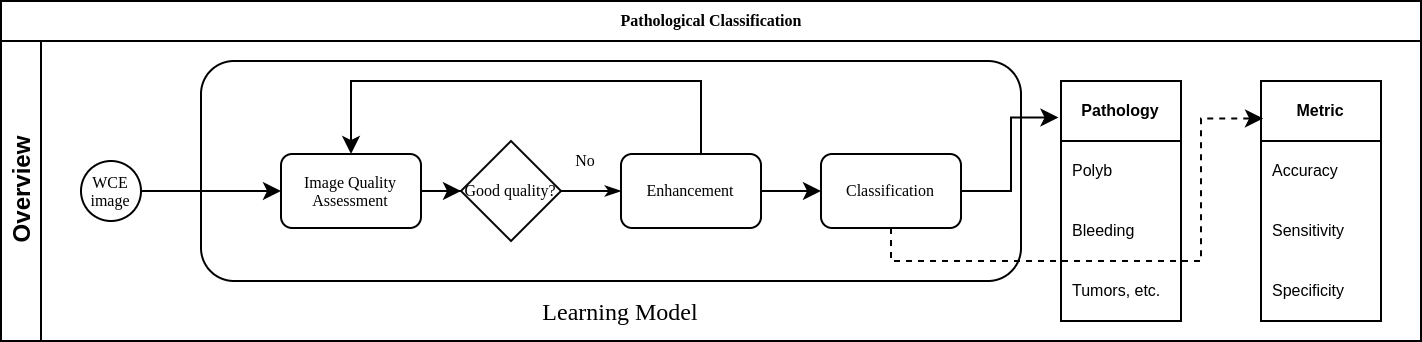
\includegraphics[scale=0.2]{libs/overallalgo.png}
        \caption{Model flowchart for overall algorithm to create a system to identify the name of pathologies}
        \label{fig:overallalgo}
    \end{figure}
    The main objective of the project is to develop a smart system for:
    \begin{itemize}
        \item Identify the pathologies on wireless capsule endoscopy (WCE) images
              \begin{itemize}
                  \item Including a pre-processing module that aims at improving the quality of the acquired images
                  \item Develop a set of image quality enhancement solutions based on kinds of distortion
              \end{itemize}


    \end{itemize}

    \vspace{0.2cm}

    There are \example{many kinds of distortion} $\&$ in \emph{different levels}
\end{frame}

\subsubsection{Challenges}
\begin{frame}{Challenges}
    % \textcolor{blue(pigment)}{\textbf{Challenges and Motivation}}\\[5pt]
    \begin{itemize}
        % \item Current challenges in the hospital: "\textcolor{red}{2 patients/day} and just \textcolor{violet}{4 working days}" 
        \item Some common acquisition distortions (\textbf{noise}, \textcolor{red}{\textbf{blur}}, \textcolor{violet}{\textbf{uneven illumination}}, \textcolor{blue}{\textbf{specular reflection}}) may affect the WCE based diagnosis.         \footnote[frame]{\tiny Borgli, H., Thambawita, V., Smedsrud, P.H. et al. \textit{HyperKvasir}, a comprehensive multi-class image and video dataset \\for gastrointestinal endoscopy. Sci Data 7, 283 (2020). https://doi.org/10.1038/s41597-020-00622-y}
    \end{itemize}


    \begin{figure}
        \centering
        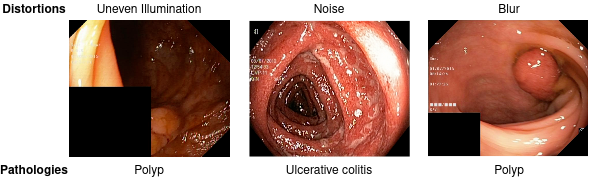
\includegraphics[scale=0.4]{libs/examdis3.png}
        % \vspace{0.4cm}
        \caption{Illustration of some common WCE images distortions. Left column: \textit{polyp} image with uneven illumination. Middle column: \textit{ulcerative colitis} image with noise. Right column: \textit{polyp} image with blur.}
        \label{fig:endoscopy}
    \end{figure}

\end{frame}

\begin{frame}
    \large How image \example{quality affects} the classification performance ?
\end{frame}

\begin{frame}{\small Effect of distortion (Blur) on the classification performace \footnote[frame]{\tiny Borel-Donohue, Christoph and S. Young. “Image quality and super resolution effects on object recognition using deep \\ neural networks.” Defense + Commercial Sensing (2019).}}
    \begin{figure}
        \centering
        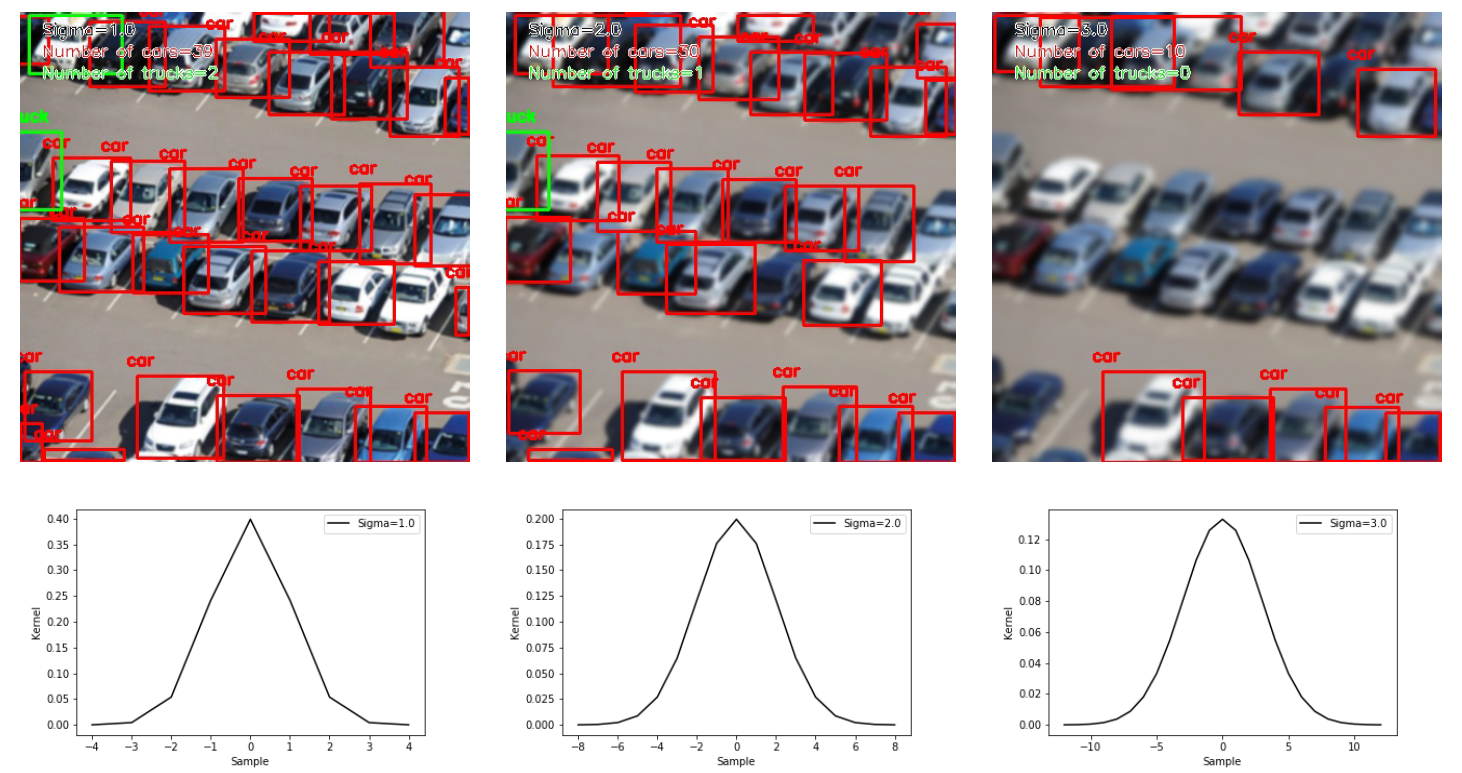
\includegraphics[scale=0.2]{libs/blureffect.png}
        % \vspace{0.4cm}
        \caption{Degradation of the vehicle detection due to image blurring. Left column: Blurred image with kernel width $\sigma=1.0$ detects 41 vehicles. Middle column: Blurred image with kernel width $\sigma=2.0$ detects 31 vehicles. Right column: Blurred image with kernel width $\sigma=3.0$ detects 10 vehicles.}       
        \label{fig:challenge}
    \end{figure}

\end{frame}

\begin{frame}{\small Effect of distortion (Noise) on the classification performace \footnote[frame]{\tiny Borel-Donohue, Christoph and S. Young. “Image quality and super resolution effects on object recognition using deep \\ neural networks.” Defense + Commercial Sensing (2019).}}
    \begin{figure}
        \centering
        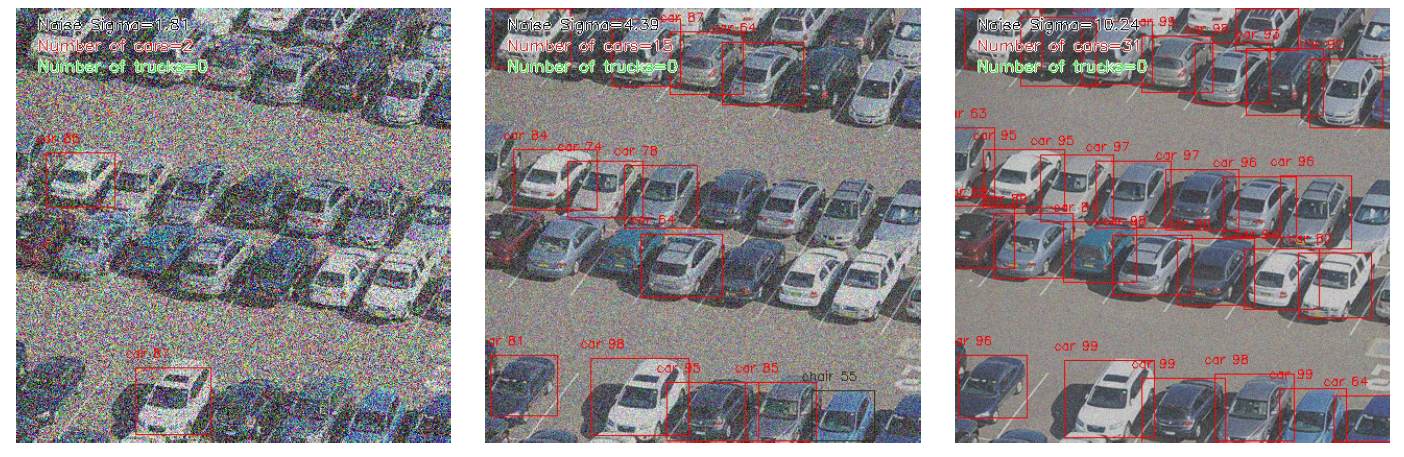
\includegraphics[scale=0.15]{libs/noiseeffect.png}
        \caption{Vehicle detections for additive noise with $SNR = {1.81, 4.39, 10.24}$.}
        \label{fig:challengenoise}
    \end{figure}
    
    \begin{figure}
        \centering
        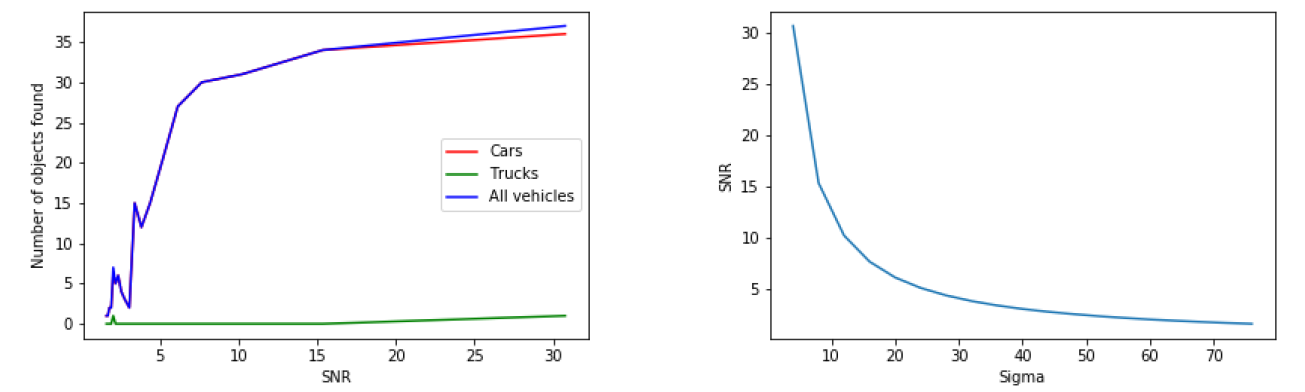
\includegraphics[scale=0.15]{libs/noiseeffect2.png}
        \caption{Number of cars detected as a function of the Gaussian noise added with a signal to noise $SNR = {1.62,..., 30.76}$. Right: SNR as a function of $\sigma = {4, 8,..., 80}$.}
        \label{fig:challengenoise2}
    \end{figure}

\end{frame}

\begin{frame}{\small Effect of distortion (Noise, Blur) on the classification performace \footnote[frame]{\tiny Dodge, Samuel F. and Lina Karam. “Understanding how image quality affects deep neural networks.” 2016 Eighth \\ International Conference on Quality of Multimedia Experience (QoMEX) (2016): 1-6.}}
    \begin{figure}
        \centering
        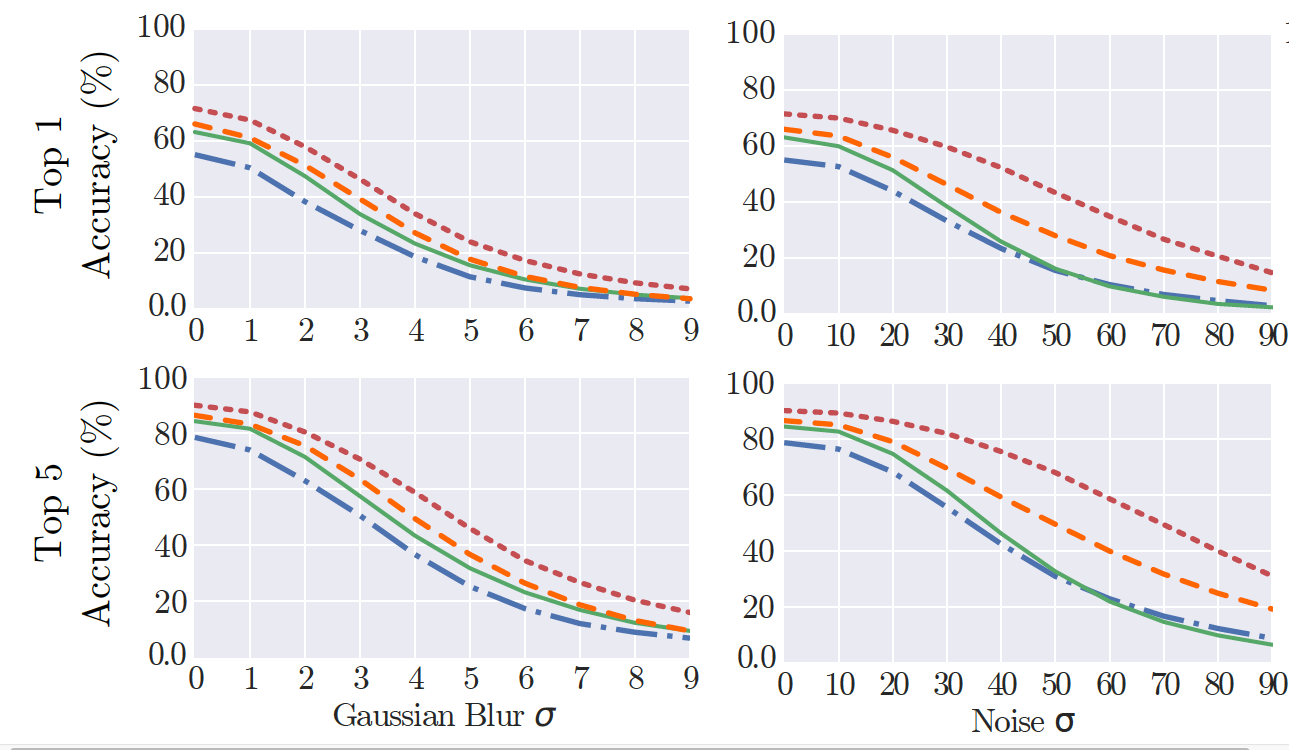
\includegraphics[scale=0.2]{libs/acceffect.png}
        \vspace{0.4cm}
        \caption{Top-1 and Top-5 Accuracy rates under different quality distortions. The networks are very sensitive to changes in blur and noise}
        \label{fig:challenge3}
    \end{figure}

\end{frame}


\subsubsection{Solutions}
%% ---------------------------------------------------------------------------
% \subsection{Subseção III}
% \begin{frame}{Algorithm}
%     % \caption{Apply the approximation quality enhancement methods}
%     \begin{algorithm}[H]

%         \SetAlgoLined
%         \LinesNumbered
%         \SetKwInOut{Input}{input}
%         \SetKwInOut{Output}{output}
%         \Input{$distorted\_image$}
%         \Output{$enhanced\_image$}
%         $types\_distortion$ = \tikzmark{classifier}{classifier} ($distorted\_image$)\;
%         \For{$type$ in $types\_distortion$}{
%             $enhanced\_image$ $\gets$ \tikzmark{enhancer}{enhancer$_{type}$} ($distorted\_image$)
%         }
%         \Return $enhanced\_image$
%         % \vspace{cao0.5cm}

%     \end{algorithm}

%     \pause
%     \tikz[overlay,remember picture]{\draw[draw=blue,thick,fill opacity=0.2] ($(classifier)+(-0.1,0.3)$) rectangle ($(classifier)+(1.3,-0.1)$);}

%     \tikz[overlay,remember picture]{\draw[draw=green,thick,fill opacity=0.2] ($(enhancer)+(-0.1,0.3)$) rectangle ($(enhancer)+(1.9,-0.2)$);}

%     \texttt{Requirement:}

%     Create the \tikz[remember picture]{ \node[anchor=base] (n1) {\tikzmark{classifier}{classifier}};} and \tikz[remember picture]{ \node[anchor=base] (n2) {\tikzmark{enhancer}{enhancer$_{type}$}};}\tikz[overlay,remember picture]{\draw[draw=blue,thick,fill opacity=0.2] ($(classifier)+(-0.1,0.3)$) rectangle ($(classifier)+(1.3,-0.1)$);}\tikz[overlay,remember picture]{\draw[draw=green,thick,fill opacity=0.2] ($(enhancer)+(-0.1,0.3)$) rectangle ($(enhancer)+(1.9,-0.2)$);}
%     \pause by using \example{learning - based} method

%     \pause
%     \vspace{0.5cm}
%     \tikz[remember picture]{ \node[fill=green!20,anchor=base] (t1) {Creating a dataset is the \emph{most important} thing to do};}
%     \begin{tikzpicture}[remember picture,overlay]   %% use here too
%         \path[draw=magenta,thick,->]<1-> (n1) to [bend right] (t1);
%         \path[draw=magenta,thick,->]<2-> (n2) to [bend left] (t1);
%     \end{tikzpicture}

% \end{frame}
\begin{frame}{Method}
    \begin{figure}
        \centering
        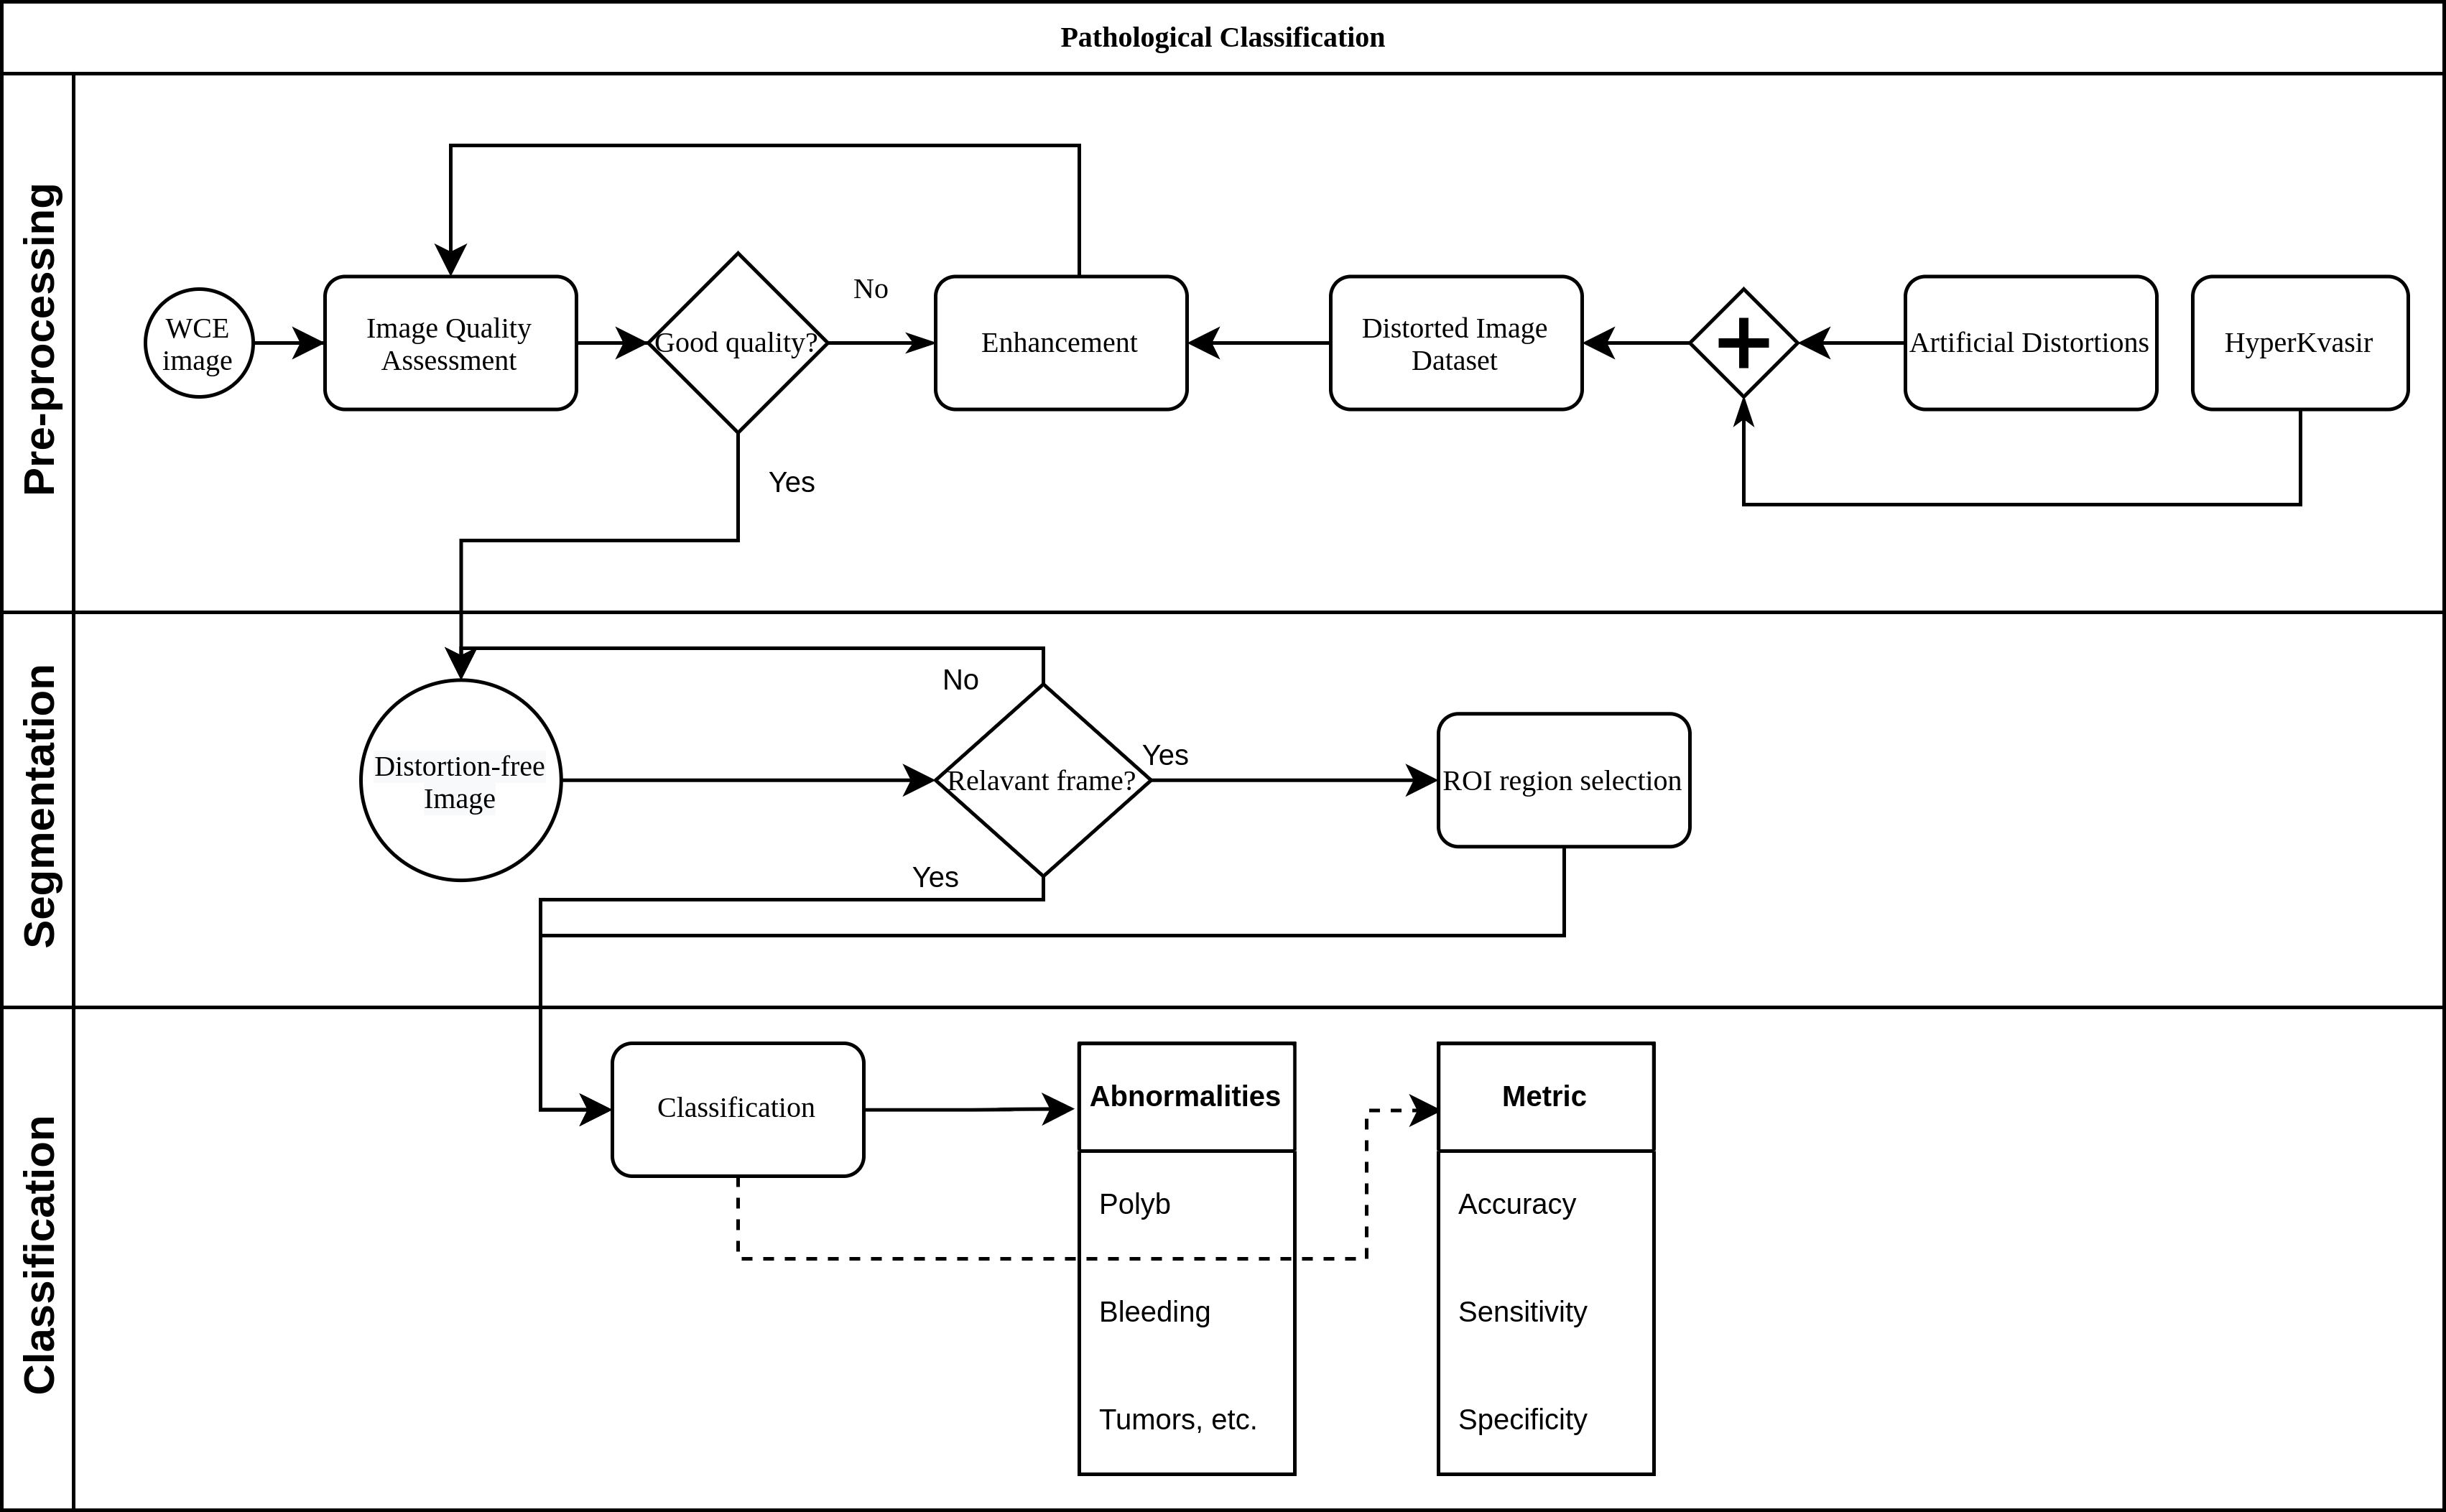
\includegraphics[scale=0.08]{libs/algorithm.png}
        \caption{ Flow chart of the pathological classification process}
        \label{fig:al}
    \end{figure}
\end{frame}

% %% ---------------------------------------------------------------------------

% \begin{frame}{Inserindo Algoritmos}
%     \lstset{language=Python}
%     \lstinputlisting[language=Python]{code/main.py}
% \end{frame}

% %% ---------------------------------------------------------------------------
% \begin{frame}{Inserindo Algoritmos}
%     \lstinputlisting[language=C]{code/source.c}
% \end{frame}

% %% ---------------------------------------------------------------------------
% \begin{frame}{Inserindo Algoritmos}
%     \lstinputlisting[language=Java]{code/helloworld.java}
% \end{frame}

% %% ---------------------------------------------------------------------------
% \begin{frame}{Inserindo Algoritmos}
%     \lstinputlisting[language=HTML]{code/index.html}
% \end{frame}

% %% ---------------------------------------------------------------------------
% % This frame show an example to insert multicolumns
\section{Existing datasets}
\subsection{Existing GI datasets}
\begin{frame}{Existing datasets}
    \begin{table}
        \caption{An overview of existing GI datasets.}
        \begin{adjustbox}{width=\textwidth}
            \begin{tabular}{|l|l|l|}
                \hline
                \rowcolor[HTML]{FFFFFF}
                \textbf{Dataset}                                                  & \textbf{Findings}                            & \textbf{Size}                     \\ \hline
                CVC-356 \cite{Bernal2012TowardsAP}                                & Polyps                                       & 356 images                        \\ \hline
                CVC-ClinicDB (also named CVC-612) \cite{Bernal2015WMDOVAMF}       & Polyps                                       & 612 images                        \\ \hline
                CVC-VideoClinicDB (also named CVC-12k) \cite{Bernal2012TowardsAP} & Polyps                                       & 11954 images                      \\ \hline
                CVC-ColonDB \cite{Bernal2012TowardsAP}                            & Polyps                                       & 380 images                        \\ \hline
                Endoscopy Artifact detection 2019 \cite{Ali2019EndoscopyAD}       & Endoscopic Artifacts                         & 5,138 images                      \\ \hline
                ASU-Mayo polyp database  \cite{Tajbakhsh2016AutomatedPD}          & Polyps                                       & 18,781 images                     \\ \hline
                ETIS-Larib Polyp DB \cite{Silva2013TowardED}                      & Polyps                                       & 196 images                        \\ \hline
                KID \cite{Koulaouzidis2017KIDPA}                                  & Angiectasia, bleeding, inflammations, polyps & 2371 images and 47 videos         \\ \hline
                GIANA 2017  \cite{Guo2019GIANAPS}                                 & Polyps \& Angiodysplasia                     & 3462 images and 38 videos         \\ \hline
                GIANA 2018  \cite{Bernal2018PolypDB}                              & Polyps \& Small bowel lesions                & 8262 images and 38 videos         \\ \hline
                GASTROLAB   \cite{gastro}                                         & GI lesions                                   & Some 100s of images andfew videos \\ \hline
                WEO Clinical Endoscopy Atlas \cite{weo}                           & GI lesions                                   & 152 images                        \\ \hline
                GI Lesions in Regular Colonoscopy Data Set \cite{uci}             & GI lesions                                   & 76 images                         \\ \hline
                Atlas of Gastrointestinal Endoscope  \cite{as72}                  & GI lesions                                   & 1295 images                       \\ \hline
                El salvador atlas of gastrointestinal video endoscopy \cite{as73} & GI lesions                                   & 5071 video clips                  \\ \hline
                Kvasir  \cite{Pogorelov2017KVASIRAM}                              & \begin{tabular}[c]{@{}l@{}} Polyps, esophagitis, ulcerative colitis, Z-line,pylorus\\ cecum, dyed polyp, dyed resection margins, stool \end{tabular}                   & 8000 images                       \\ \hline
                Kvasir-SEG   \cite{Jha2020KvasirSEGAS}                            & Polyps                                       & 1000 images                       \\ \hline
                Nerthus  \cite{Pogorelov2017NerthusAB}                            & Stool - categorization of bowel cleanliness  & 21 videos                         \\ \hline
            \end{tabular}
        \end{adjustbox}

    \end{table}
    \pause
    \alertbox{They are rather small, and often limited to polyps. Several of these have also lately become unavailable.\tikz[remember picture]{ \node[anchor=base] (n3) {};}}
    \pause
    \tikz[remember picture]{ \node[fill=green!20,anchor=base] (t3) {Using \emph{HyperKvasir} \cite{Borgli2020HyperKvasirAC} dataset};}
    \begin{tikzpicture}[remember picture,overlay]   %% use here too
        \path[draw=magenta,thick,->]<1-> (n3) to [bend right] (t3);
    \end{tikzpicture}
\end{frame}
\subsection{HyperKvasir dataset}
\begin{frame}{HyperKvasir dataset}
    \begin{table}[]
        \caption{Overview of the data records in the HyperKvasir dataset.}
        \begin{adjustbox}{width=\textwidth}
            \begin{tabular}{|l|l|l|}
                \hline
                \multicolumn{1}{|c|}{\textbf{Data Record}}                          & \multicolumn{1}{c|}{\textbf{\# Files}} & \multicolumn{1}{c|}{\textbf{Description}} \\ \hline
                \tikz[remember picture]{ \node[anchor=base] (n4) {};}Labeled images & 10,662 images                          & 23 classes of findings                    \\ \hline
                Segmented Images                                                    & 1,000 images                           & Segmentation masks for polyp findings     \\ \hline
                Unlabeled Images                                                    & 99,417 images                          & Unlabeled                                 \\ \hline
                \tikz[remember picture]{ \node[anchor=base] (n5) {};}Videos         & 374 videos                             & 30 different classes                      \\ \hline
            \end{tabular}
        \end{adjustbox}
    \end{table}
    \pause

    \begin{figure}
        \centering
        \tikz[remember picture]{ \node[anchor=base] (t4) {};}
        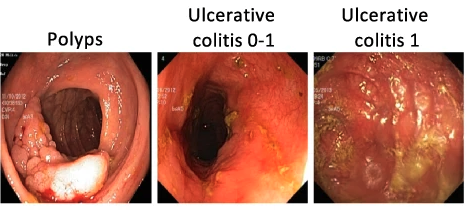
\includegraphics[scale=0.1]{libs/hyperkvasir_ex.png}
        \caption{Image examples of the various labeled classes for images and/or videos.}
    \end{figure}
    \begin{tikzpicture}[remember picture,overlay]   %% use here too
        \path[draw=magenta,thick,->]<1-> (n4) to [bend right] (t4);
        \path[draw=blue,thick,->]<1-> (n5) to [bend right] (t4);
    \end{tikzpicture}
\end{frame}
%% ---------------------------------------------------------------------------
% This frame show an example to insert figures
\section{Our work}
\subsection{Method}
\tikzset{
    vertex/.style = {
            circle,
            fill            = black,
            outer sep = 2pt,
            inner sep = 1pt,
        }
}
\begin{frame}{Ourwork}
    \example{Our work} has three stages including cleaning the existing distortion in HyperKvasir dataset, then we create the model to generate the new artificial distortions. Finally, we add the new artificial distortions to the antidistorted images.\\
    \begin{tikzpicture}
        % Dialectics
        \node[draw] (Original) at (0,2) {Original};
        \node[draw,fill=black,text=white] (Antidistortion) at (2.3,2) {Antidistortion};
        \node[draw,fill=gray,text=white] (Cleaner) at (1,4) {Cleaner};

        \draw node[vertex] (Joint) at (1,2) {};

        \draw[-,draw=blue] (Original) to (Joint);
        \draw[-,draw=blue] (Antidistortion) to (Joint);
        \draw[->,draw=blue] (Joint) to (Cleaner);
        \draw[->,draw=blue] (Cleaner) to[in=180,out=180] (Original);
        \node at (1.0, 1.0) {\textit{a) Clean the image}};
        % \onslide<1,2>{\node (step1)  at (3,-1){   \example{Step 1} Cleaning the existing distortion in HyperKvasir dataset};}
        % \pause
        % \onslide<2>{
        %     \node (example)  at (7,2){                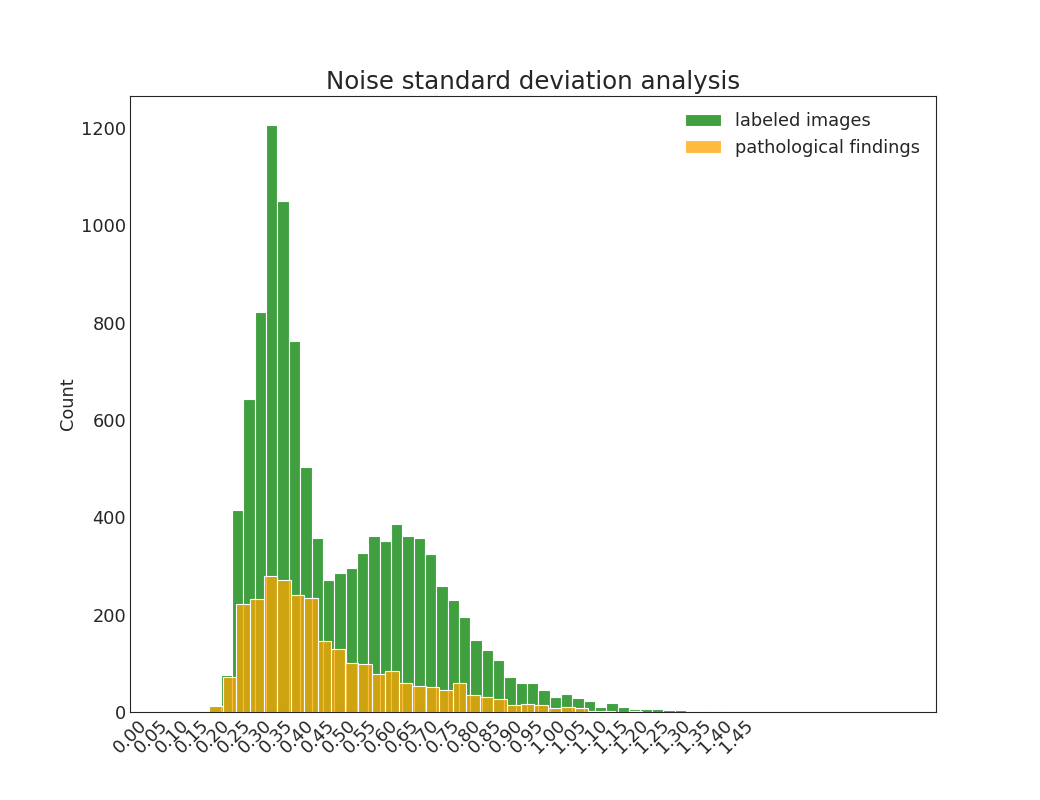
\includegraphics[width=0.5\columnwidth]{libs/sigmahist.png} };
        %     \draw[->,draw=red] (example) to (Cleaner);


        % }


        % \pause
        % Opposition
        \node[draw] (ArgumentA) at (5,2) {Distortion};
        \node[draw,fill=yellow] (ArgumentB) at (7.5,2) {Model};

        \draw[->,draw=blue] (ArgumentA) to (ArgumentB);

        \node at (6., 1.0) {\textit{b) Create model}};
        % \onslide<3>{\node (step2)  at (3,-1){   \example{Step 2} Creating the model to generate the new artificial distortions};}
        % \pause
        % \onslide<4>{
        %     \node (old)  at (5,4){                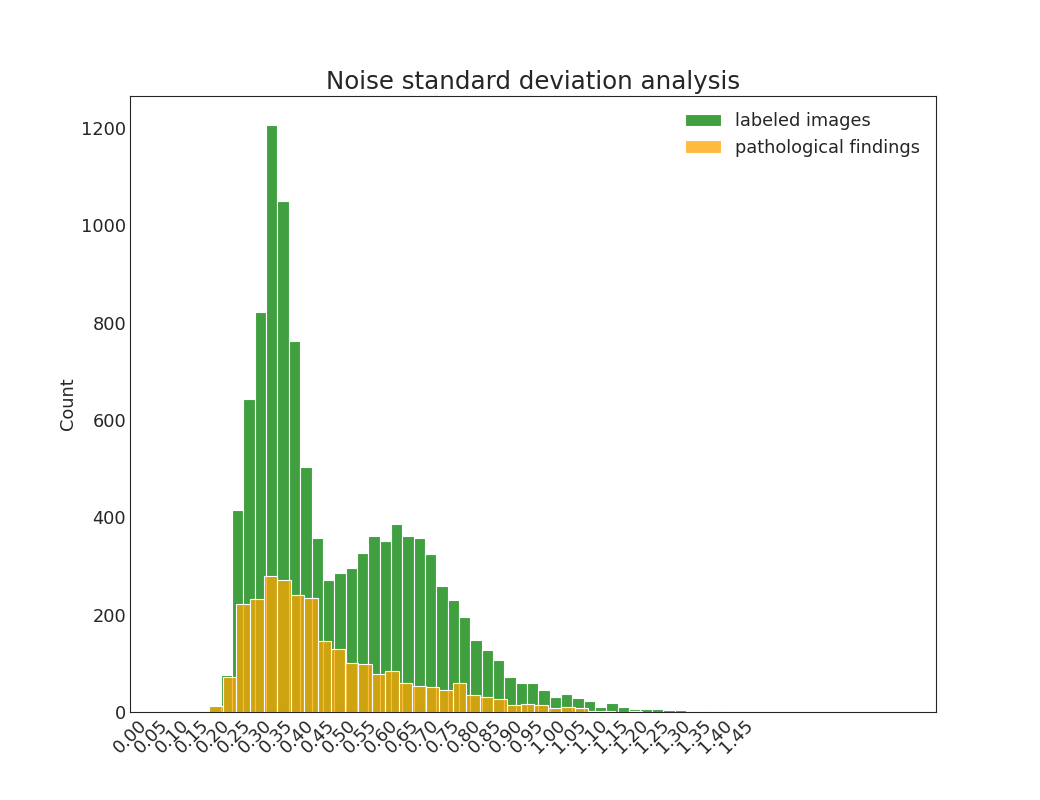
\includegraphics[width=0.2\columnwidth]{libs/sigmahist.png} };
        %     \draw[->,draw=yellow] (old) [bend left] to (ArgumentB);
        %     \node (example)  at (4,-1){
        %         
\includegraphics[width=0.2\columnwidth]{libs/sb_mask.png} };
        %     \draw[->,draw=red] (example) [bend right] to (ArgumentB);
        % }
        % \pause
        % Innovation
        \node[draw,fill=black,text=white] (ArgumentA) at (2.1,-0.5) {Antidistortion};
        \node[draw,fill=violet,text=white] (ArgumentB) at (5.3,-0.5) {Results};
        \node[draw,fill=yellow] (ArgumentC) at (3,0.5) {Model};

        \draw node[vertex] (Joint) at (3.6,-0.5) {};

        \draw[-] (ArgumentA) to (Joint);
        \draw[-] (ArgumentB) to (Joint);
        \draw[->,draw=blue] (ArgumentC) to (Joint);

        \node at (3.5, -1.5) {\textit{c) Add artificial distortion}};
        % \onslide<5>{\node (step2)  at (3,5){   \example{Step 3} Add the new artificial distortions to the antidistorted images};}
    \end{tikzpicture}
\end{frame}


\subsection{Results}
\begin{frame}{Results}
    \example{Stage 1:} we have to clean the existing distortion in the HyperKvasir dataset.\\ 
    \begin{tikzpicture}[remember picture]
        \node[draw] (input) at (-1,-4) {Original Image};
        \node[draw,fill=yellow] (noise) at (1.5,-4) {Denoising}; %% use here too
        \path[draw=magenta,thick,->]<1-> (input) to [bend right] (noise);

        \node[draw] (blur) at (3.5,-4) {Debluring};
        \path[draw=magenta,thick,->]<1-> (noise) to [bend left] (blur);

        \node[draw,fill=yellow] (uneven) at (6.3,-6) {Uneven Illumination Correction};
        \path[draw=magenta,thick,->]<1-> (blur) to [bend left] (uneven);

        \node[draw,fill=white] (sr) at (0,-6) {Specular Reflection Removal};
        \path[draw=magenta,thick,->]<1-> (uneven) to  (sr);

        \node[draw,fill=black, text = white] (anti) at (0,-8) {Antidistorted Image};
        \path[draw=magenta,thick,->]<1-> (sr) to  (anti);

        \node[draw,fill=gray] (add) at (6,-8) {Artificial Distortion Model};
        \path[draw=magenta,thick,->,dashed]<1-> (anti) to  (add);

    \end{tikzpicture}
\end{frame}
% \begin{frame}{Results}

%     \begin{itemize}
%         \only<1-5>{\item Noise
%               \only<1-4>{
%                   \begin{tikzpicture}[remember picture]

%                       \node (in)  at (-3,0){
%                           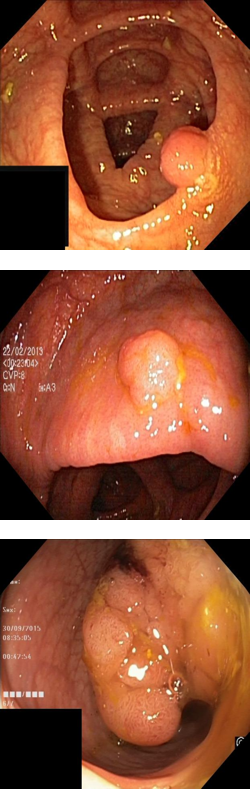
\includegraphics[width=0.15\columnwidth]{libs/input.png} };
%                       \node at (-3.0, -3.0) {\small\textit{a) Original}};
%                       \pause
%                       \node (noisy1)  at (-1,0){
%                           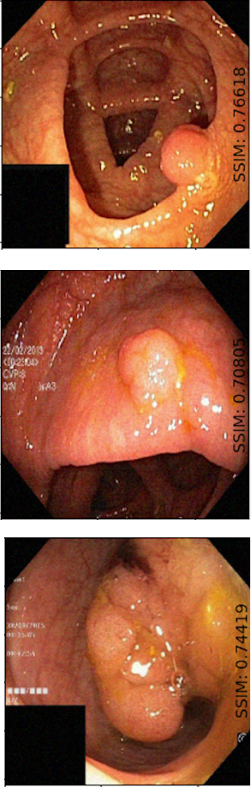
\includegraphics[width=0.15\columnwidth]{libs/noisy.png} };
%                       \node at (-1.0, -3.0) {\small\textit{b) Noisy}};
%                       \path[draw=magenta,thick,->]<1-> (in) to  (noisy1);
%                       \pause
%                       \node (denoised1)  at (1,0){
%                           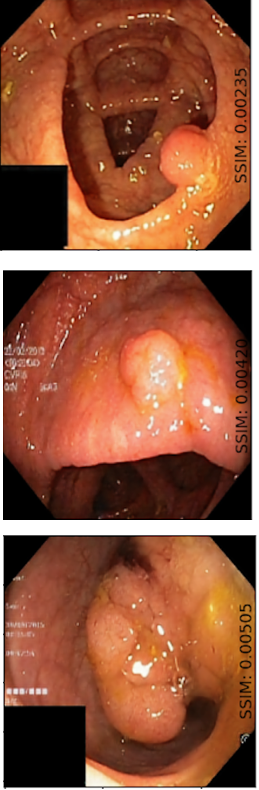
\includegraphics[width=0.15\columnwidth]{libs/denoised.png} };
%                       \node at (1.0, -3.0) {\small\textit{c) Denoised}};
%                       \path[draw=magenta,thick,->]<1-> (noisy1) to  (denoised1);
%                       \pause
%                       \node (tabnoise)  at (4.5,0){
%                           \begin{adjustbox}{width=0.45\textwidth}
%                               \begin{tabular}{|c|l|c|l|c|l|c|l|c|l|c|l|}
%                                   \hline
%                                   \multicolumn{4}{|c|}{}                            & \multicolumn{2}{c|}{\textbf{Noisy-image}} & \multicolumn{2}{c|}{\textbf{C-BM3D}} & \multicolumn{2}{c|}{\textbf{NM-Mean}} & \multicolumn{2}{c|}{\textbf{CAE}}                                        \\ \hline
%                                   \multicolumn{2}{|c|}{\multirow{7}{*}{$\sigma_n$}} & \multicolumn{2}{c|}{0.25}                 & \multicolumn{2}{c|}{0.8095}          & \multicolumn{2}{c|}{0.7364}           & \multicolumn{2}{c|}{0.9068}       & \multicolumn{2}{c|}{\textbf{0.9158}} \\ \cline{3-12}
%                                   \multicolumn{2}{|c|}{}                            & \multicolumn{2}{c|}{0.3}                  & \multicolumn{2}{c|}{0.7561}          & \multicolumn{2}{c|}{0.7275}           & \multicolumn{2}{c|}{0.8884}       & \multicolumn{2}{c|}{\textbf{0.9097}} \\ \cline{3-12}
%                                   \multicolumn{2}{|c|}{}                            & \multicolumn{2}{c|}{0.35}                 & \multicolumn{2}{c|}{0.7084}          & \multicolumn{2}{c|}{0.7106}           & \multicolumn{2}{c|}{0.8752}       & \multicolumn{2}{c|}{\textbf{0.9033}} \\ \cline{3-12}
%                                   \multicolumn{2}{|c|}{}                            & \multicolumn{2}{c|}{0.4}                  & \multicolumn{2}{c|}{0.6615}          & \multicolumn{2}{c|}{0.7039}           & \multicolumn{2}{c|}{0.8614}       & \multicolumn{2}{c|}{\textbf{0.8991}} \\ \cline{3-12}
%                                   \multicolumn{2}{|c|}{}                            & \multicolumn{2}{c|}{0.6}                  & \multicolumn{2}{c|}{0.5102}          & \multicolumn{2}{c|}{0.6517}           & \multicolumn{2}{c|}{0.8222}       & \multicolumn{2}{c|}{\textbf{0.8766}} \\ \cline{3-12}
%                                   \multicolumn{2}{|c|}{}                            & \multicolumn{2}{c|}{0.65}                 & \multicolumn{2}{c|}{0.4810}          & \multicolumn{2}{c|}{0.6428}           & \multicolumn{2}{c|}{0.8132}       & \multicolumn{2}{c|}{\textbf{0.8681}} \\ \cline{3-12}
%                                   \multicolumn{2}{|c|}{}                            & \multicolumn{2}{c|}{0.7}                  & \multicolumn{2}{c|}{0.4508}          & \multicolumn{2}{c|}{0.6389}           & \multicolumn{2}{c|}{0.8051}       & \multicolumn{2}{c|}{\textbf{0.8661}} \\ \hline
%                               \end{tabular}
%                           \end{adjustbox}};
%                       \node[text width=5cm] at (4.5, -2.0) {\small\textit{d) Comparison using mean SSIM for different level where $n \sim N(0, \sigma^2_n)$}};
%                   \end{tikzpicture}}
%               \pause
%               \only<5>{
%                   \begin{table}[h]
%                       \centering
%                       \caption{Comparison using mean SSIM for different level where $n \sim N(0, \sigma^2_n)$}
%                       \label{ssimcom}
%                       \begin{adjustbox}{width=0.8\textwidth}
%                           \begin{tabular}{|c|c|c|c|c|c|c|c|}
%                               \hline
%                                                    & \multicolumn{7}{c|}{\textbf{$\sigma_n$}}                                                                                                             \\ \hline
%                                                    & 0.25                                     & 0.3             & 0.35            & 0.4             & 0.6             & 0.65            & 0.7             \\ \hline
%                               \textbf{Noisy-image} & 0.8095                                   & 0.7561          & 0.7084          & 0.6615          & 0.5102          & 0.4810          & 0.4508          \\ \hline
%                               \textbf{C-BM3D}      & 0.7364                                   & 0.7275          & 0.7106          & 0.7039          & 0.6517          & 0.6428          & 0.6389          \\ \hline
%                               \textbf{NM-Mean}     & 0.9068                                   & 0.8884          & 0.8752          & 0.8614          & 0.8222          & 0.8132          & 0.8051          \\ \hline
%                               \textbf{CAE}         & \textbf{0.9158}                          & \textbf{0.9097} & \textbf{0.9033} & \textbf{0.8991} & \textbf{0.8766} & \textbf{0.8681} & \textbf{0.8661} \\ \hline
%                           \end{tabular}
%                       \end{adjustbox}
%                   \end{table}

%                   \begin{table}[h]
%                       \centering
%                       \caption{Comparison using mean PSNR for different level where $n \sim N(0, \sigma^2_n)$}
%                       \label{psnrcom}
%                       \begin{adjustbox}{width=0.8\textwidth}
%                           \begin{tabular}{|c|c|c|c|c|c|c|c|}
%                               \hline
%                                                    & \multicolumn{7}{c|}{\textbf{$\sigma_n$}}                                                                                                       \\ \hline
%                                                    & 0.25                                     & 0.3            & 0.35           & 0.4            & 0.6            & 0.65           & 0.7            \\ \hline
%                               \textbf{Noisy-image} & 32.89                                    & 31.44          & 30.34          & 29.32          & 26.37          & 25.85          & 25.22          \\ \hline
%                               \textbf{C-BM3D}      & 27.51                                    & 27.52          & 27.47          & 27.47          & 27.28          & 27.21          & 27.16          \\ \hline
%                               \textbf{NM-Mean}     & \textbf{35.81}                           & \textbf{34.74} & \textbf{34.12} & \textbf{33.48} & \textbf{31.85} & \textbf{31.51} & 31.14          \\ \hline
%                               \textbf{CAE}         & 32.28                                    & 32.56          & 32.70          & 32.38          & 31.42          & 31.18          & \textbf{31.43} \\ \hline
%                           \end{tabular}
%                       \end{adjustbox}
%                   \end{table}
%               }}


%     \end{itemize}
% \end{frame}

\begin{frame}{Results on Image denoising}
    For an image $I$ with width $W$ and height $H$, the estimated standard deviation $\sigma_n$ of noise is estimated as\footnote[frame]{Immerkær, John. “Fast Noise Variance Estimation.” Comput. Vis. Image \\ Underst. 64 (1996): 300-302.}:
\begin{equation}
    \sigma_n = \sqrt{\frac{\pi}{2}}\frac{1}{6(W-2)(H-2)}\sum_{x,y}|{I(x,y)*M_N}|
\end{equation}
    where $M_N = 2(L_2-L_1)$ with the given $L_1, L_2$:
\begin{equation}
    L_1 = \begin{bmatrix}
0 & 1 & 0\\
1 & -4 & 1\\
0 & 1 & 0
\end{bmatrix}
\end{equation}
\begin{equation}
    L_2 = \begin{bmatrix}
1 & 0 & 1\\
0 & -4 & 0\\
1 & 0 & 1
\end{bmatrix}
\end{equation}

\end{frame}


\begin{frame}{Results on Image denoising}
\begin{figure}
\centering
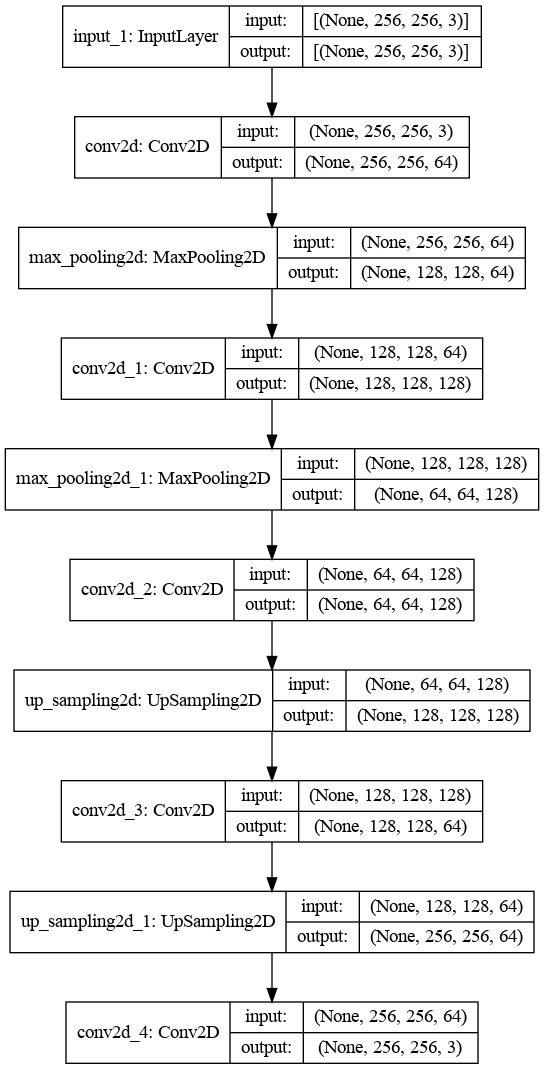
\includegraphics[width=0.3\textwidth]{libs/model.png}
\caption{The Autoencoder model used for denoising}
\end{figure}

\end{frame}

\begin{frame}{Results on Image denoising}

    % \begin{itemize}
        % \only<1-4>{\item Blur\\
              \only<1-3>{
                  \begin{tikzpicture}[remember picture]

                      \node (in)  at (-3,0){
                          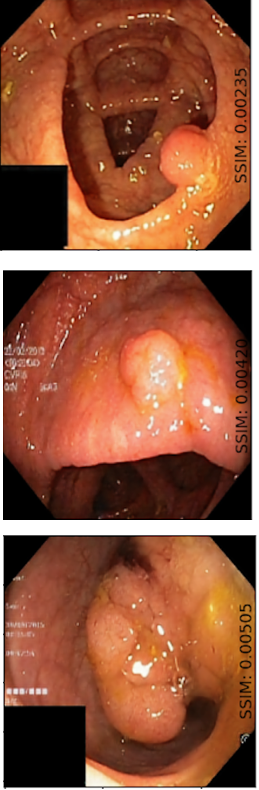
\includegraphics[width=0.15\columnwidth]{libs/denoised.png} };
                      \node at (-3.0, -3.0) {\small\textit{a) Original image}};
                      \pause
                      \node (noisy1)  at (0,0){
                          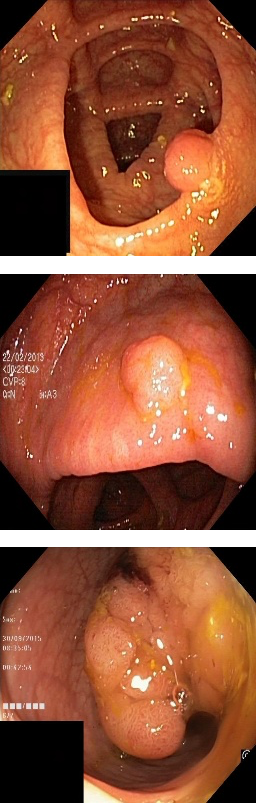
\includegraphics[width=0.15\columnwidth]{libs/deblured.png} };
                      \node at (0.0, -3.0) {\small\textit{b) Denoised image}};
                      \path[draw=magenta,thick,->]<1-> (in) to  (noisy1);
                      \pause
                      \only<3>{
                          \node (tabnoise)  at (4,0){
                              \begin{adjustbox}{width=0.5\textwidth}
                                  \begin{tabular}{|l|c|l|c|l|}
                                      \hline
                                                                   & \multicolumn{2}{c|}{\textbf{Original image}} & \multicolumn{2}{c|}{\textbf{Deblured- mage}} \\ \hline
                                      \textit{\textbf{First exp}}  & \multicolumn{2}{c|}{0.75}                     & \multicolumn{2}{c|}{0.7}                     \\ \hline
                                      \textit{\textbf{Second exp}} & \multicolumn{2}{c|}{1.45}                     & \multicolumn{2}{c|}{0.96}                     \\ \hline
                                      \textit{\textbf{Third exp}}  & \multicolumn{2}{c|}{1.1}                     & \multicolumn{2}{c|}{0.90}                     \\ \hline
                                  \end{tabular}
                              \end{adjustbox}};
                          \node[text width=5cm] at (3.5, -2.0) {\small{\textcolor{blue_theme}{Table 5:} The estimated noise standard deviation before and after denoising.}};

                      }
                  \end{tikzpicture}}
            %   }


    % \end{itemize}
\end{frame}

\begin{frame}{Results on Image deblurring}
    \begin{figure}
    \centering
    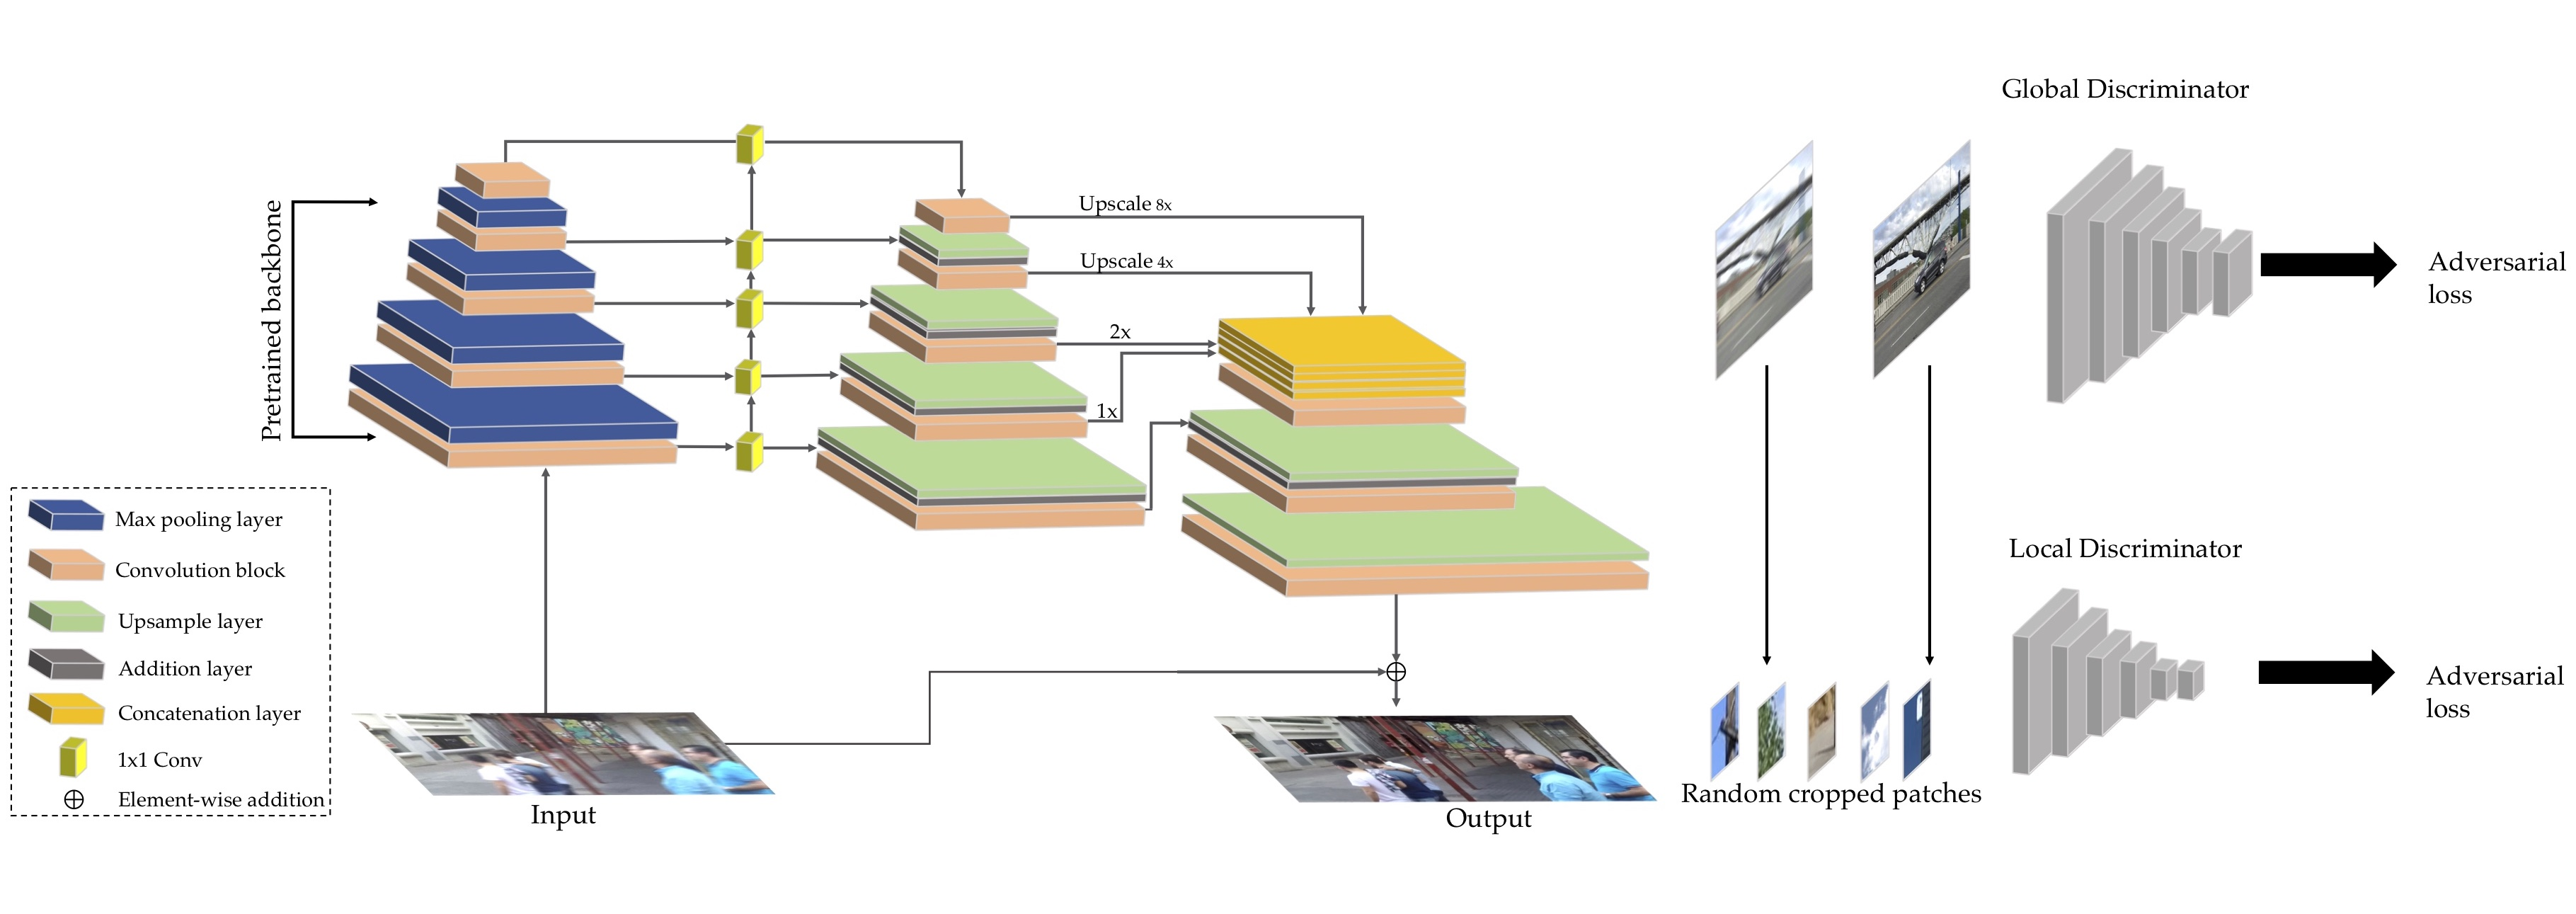
\includegraphics[width=1\textwidth]{libs/pipeline.jpg}
    \caption{The DeblurGAN v2 model used for deblurring \cite{Kupyn2019DeblurGANv2D}}
    \end{figure}
    
    \end{frame}

\begin{frame}{Results on Image deblurring}

    \begin{itemize}
        \only<1-4>{\item Blur\\
              \only<1-4>{
                  \begin{tikzpicture}[remember picture]

                      \node (in)  at (-3,0){
                          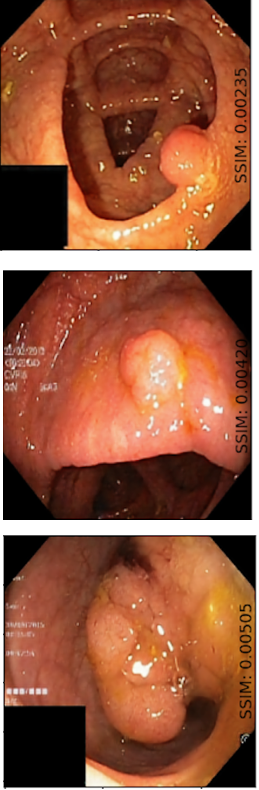
\includegraphics[width=0.15\columnwidth]{libs/denoised.png} };
                      \node at (-3.0, -3.0) {\small\textit{a) Denoised}};
                      \pause
                      \node (noisy1)  at (-1,0){
                          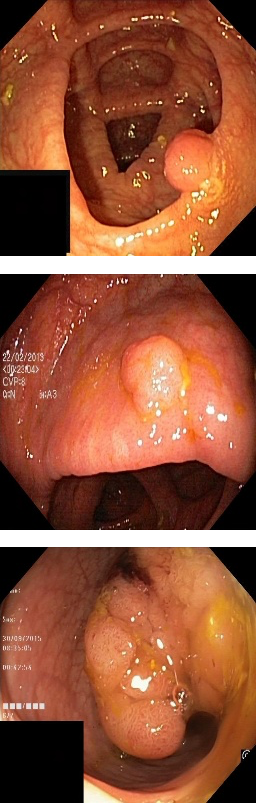
\includegraphics[width=0.15\columnwidth]{libs/deblured.png} };
                      \node at (-1.0, -3.0) {\small\textit{b) Deblurred}};
                      \path[draw=magenta,thick,->]<1-> (in) to  (noisy1);
                      \pause
                      \only<3>{\node (equablur)  at (3.5,0){
                              $\begin{aligned}
                                      index = var(\mathcal{L}(f(x,y)))
                                  \end{aligned}$};
                          \node[text width=5.5cm] at (3.5, -2.0) {\small\textit{Apply the \example{variance of the Laplacian}\cite{Pertuz2013AnalysisOF} method to your own photos to detect the amount of blurring.}};
                      }
                      \pause
                      \only<4>{
                          \node (tabnoise)  at (3.5,0){
                              \begin{adjustbox}{width=0.5\textwidth}
                                  \begin{tabular}{|l|c|l|c|l|}
                                      \hline
                                                                   & \multicolumn{2}{c|}{\textbf{Denoised-image}} & \multicolumn{2}{c|}{\textbf{Deblured- mage}} \\ \hline
                                      \textit{\textbf{First exp}}  & \multicolumn{2}{c|}{378}                     & \multicolumn{2}{c|}{501}                     \\ \hline
                                      \textit{\textbf{Second exp}} & \multicolumn{2}{c|}{321}                     & \multicolumn{2}{c|}{428}                     \\ \hline
                                      \textit{\textbf{Third exp}}  & \multicolumn{2}{c|}{224}                     & \multicolumn{2}{c|}{367}                     \\ \hline
                                  \end{tabular}
                              \end{adjustbox}};
                          \node[text width=5cm] at (3.5, -2.0) {\small{\textcolor{blue_theme}{Table 5:} The variance Laplacian Index before and after deblurring.}};

                      }
                  \end{tikzpicture}}
              }


    \end{itemize}
\end{frame}


\begin{frame}{Results on Uneven Illumination Correction}

    \begin{figure}
        \centering
        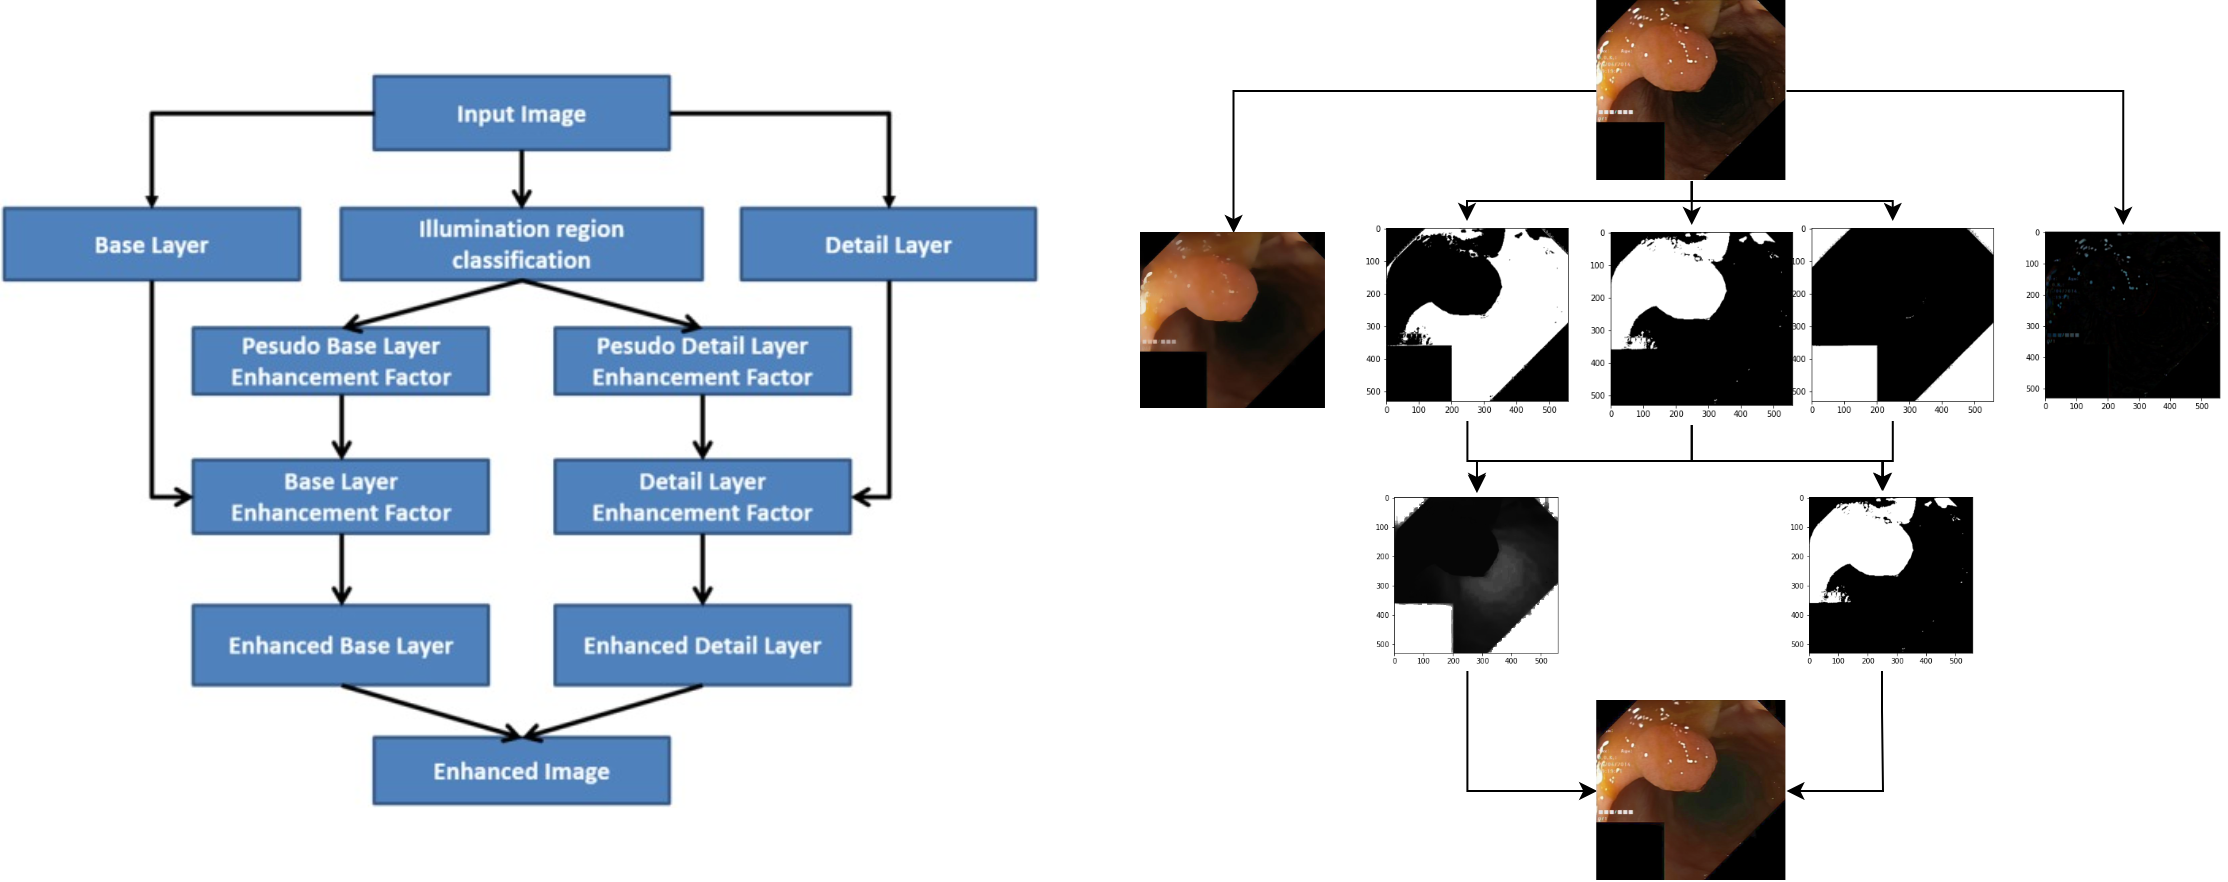
\includegraphics[width=1\textwidth]{libs/illres.png}
        \caption{Uneven Illumination Correction process using \cite{Xia2018EndoscopicIE}}
        \label{uneven_illumination_correction}
    \end{figure}
\end{frame}

\begin{frame}

        \begin{figure}
            \centering
            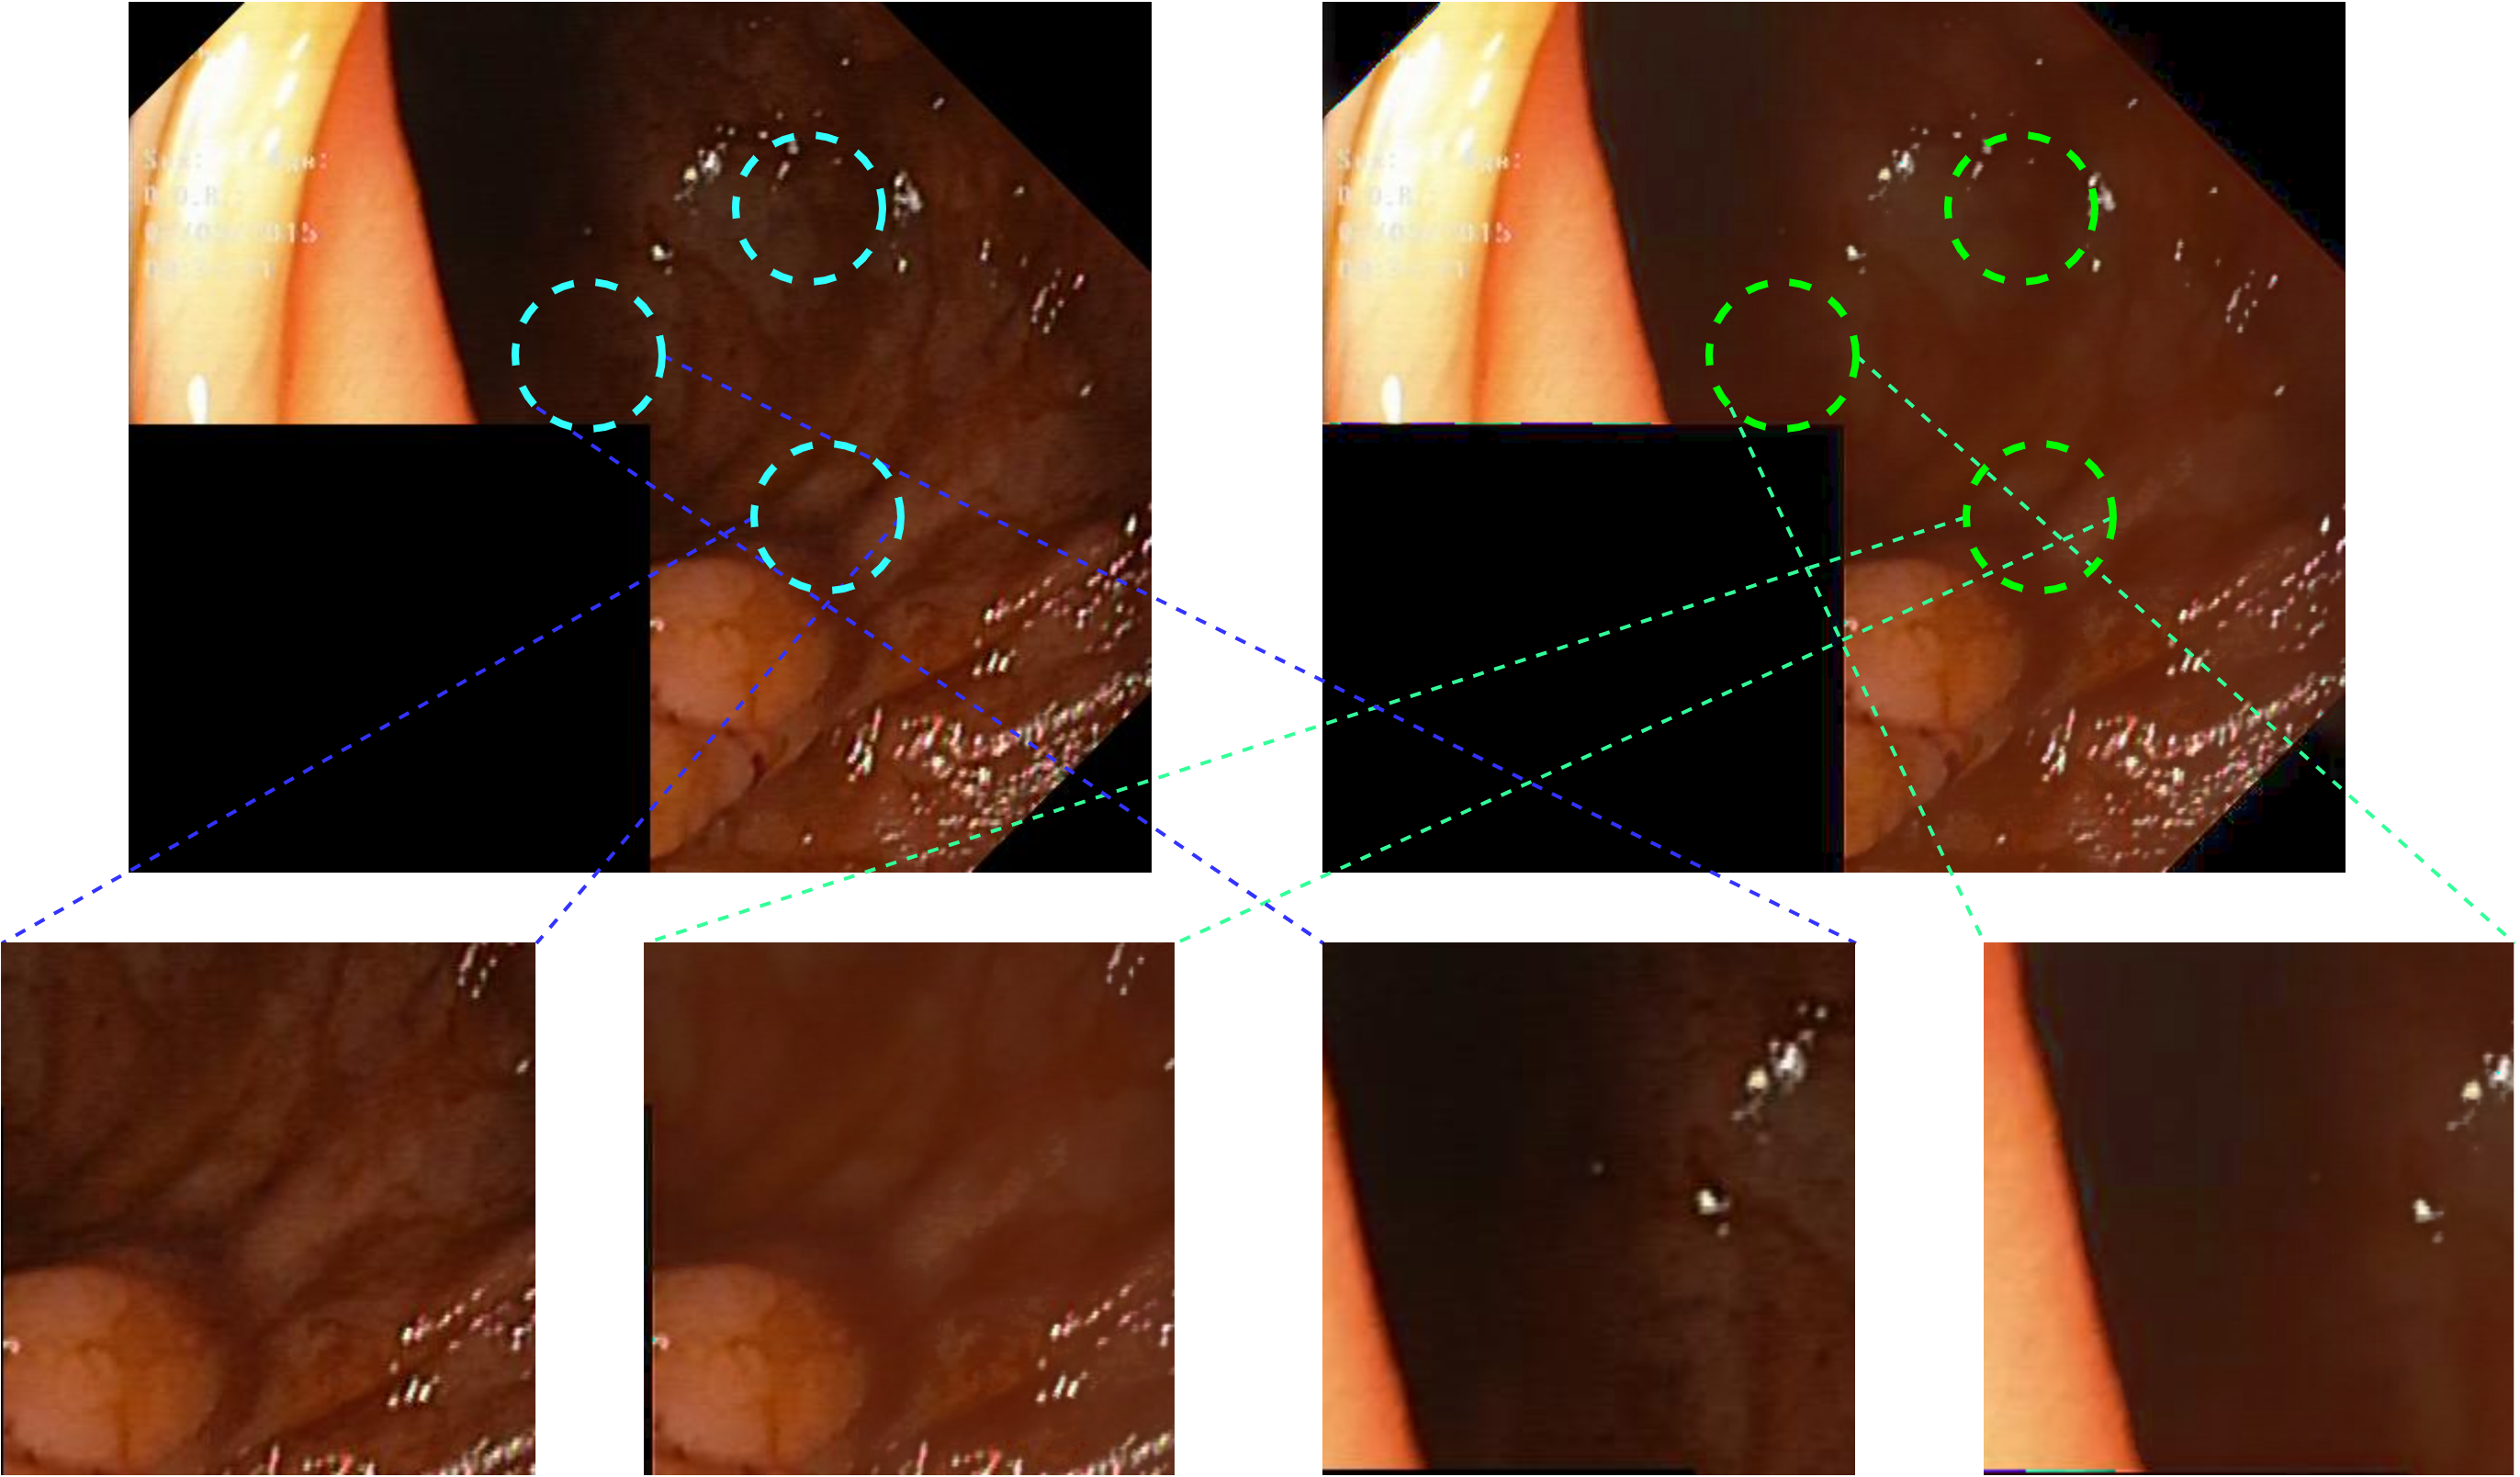
\includegraphics[width=1\textwidth]{libs/illres2.png}
            \caption{Uneven Illumination Correction result. The first row is the original image with the some uneven illmination region (red circle). In the second column, these regions have been corrected (green circle)}
            \label{uneven_illumination_correction2}
        \end{figure}
\end{frame}

\begin{frame}{Results on Specular Reflection Removal}

\begin{figure}
    \centering
    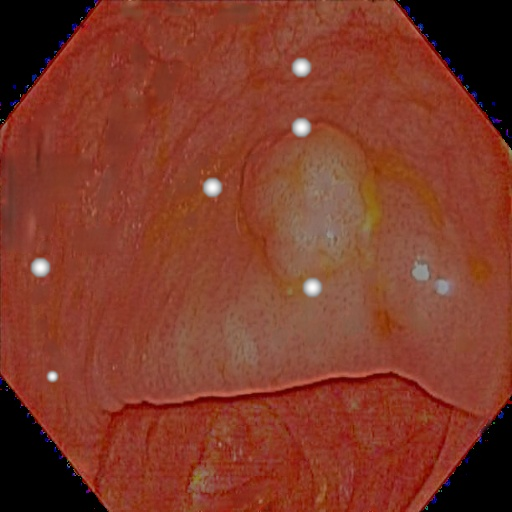
\includegraphics[width=1\textwidth]{libs/srres.png}
    \caption{Specular Reflection Removal result. First columns: the input image with specular references. The third column is the result of the Specular Reflection inpainted image using the SR mask (second column) insprired from \cite{yi2020contextual}.} 
\end{figure}
\end{frame}

\begin{frame}{Results}

    \begin{tikzpicture}[remember picture]

        \node[text width=10cm](text) at (0,2) {In this work, we create a model to add the artificial distortion to the image. There will be \example{four} different models corresponding to four kinds of distortions. We analysed the common level of distortion to simulate to realest artificial distortion which will make the dataset meaningful.};

        \node[draw,fill=black, text = white] (anti) at (-2,0) {Antidistorted Image};
        \pause
        \node[draw,fill=gray] (add) at (3,0) {Artificial Distortion Model};
        \path[draw=magenta,thick,->,dashed]<1-> (anti) to  (add);
        \pause
        \node[draw,fill=yellow] (res) at (3,-2) {Results};
        \path[draw=magenta,thick,->]<1-> (add) to  (res);



    \end{tikzpicture}
\end{frame}


\begin{frame}{Result images after adding Noise}

    % % \begin{itemize}
    %     % \only<1-3>{\item Noise\\
    %           \only<1-3>{
    %               \begin{tikzpicture}[remember picture]

    %                   \node (in)  at (-3,0){
    %                       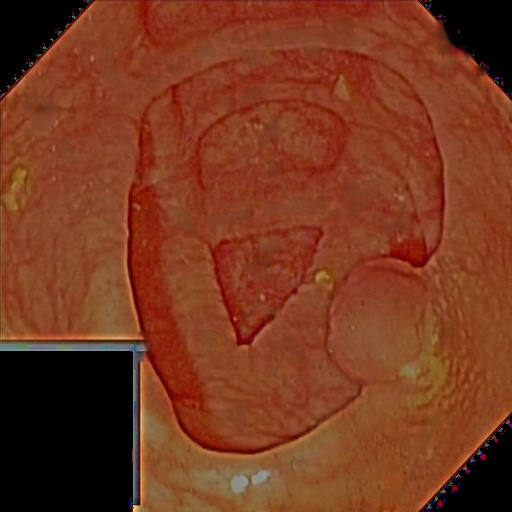
\includegraphics[width=0.25\columnwidth]{libs/out2.png_inpainted.jpg} };
    %                   \node[text width=2.5cm] at (-3.0, -3.0) {\small\textit{a) Antidistorted Image}};
    %                   \pause
    %                   \node (ref1)  at (0,0){
    %                       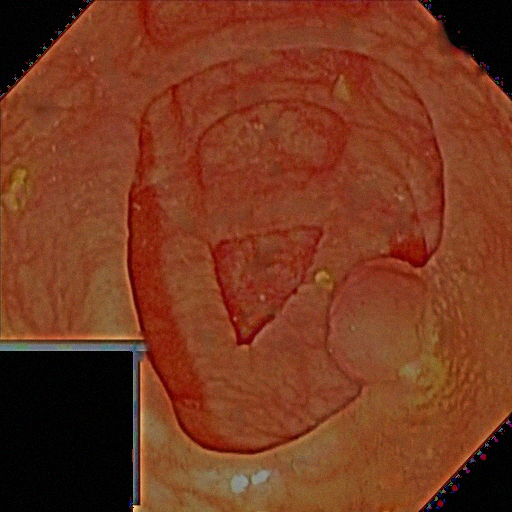
\includegraphics[width=0.25\columnwidth]{libs/AWGN_var_0.0005.png} };
    %                   \path[draw=magenta,thick,->]<1-> (in) to  (ref1);
    %                   \node[text width=2.5cm] at (0.0, -3.0) {\small\textit{b) Noised image with Gaussian Noise $n \sim N(0, \sigma^2_n=(0.0005)^2)$ }};
    %                   \pause
    %                   \node (noisy1)  at (3,0){
    %                       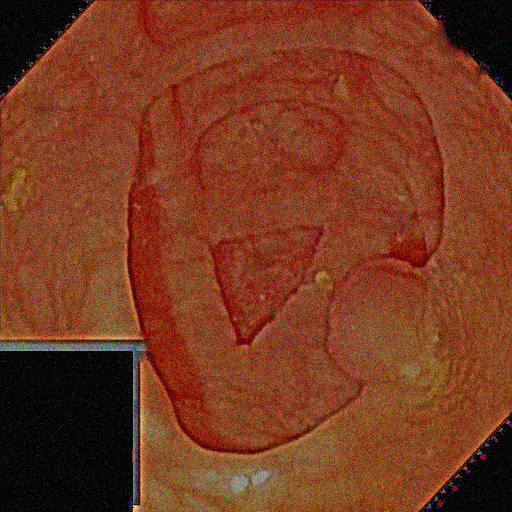
\includegraphics[width=0.25\columnwidth]{libs/AWGN_var_0.005.png} };
    %                   \node[text width=2.5cm] at (3.0, -3.0) {\small\textit{c) Noised image with Gaussian Noise $n \sim N(0, \sigma^2_n=(0.005)^2)$ }};
    %                   \path[draw=magenta,thick,->]<1-> (in) to [bend right] (noisy1);


    %               \end{tikzpicture}}
    %         %   }


    % % \end{itemize}
    \begin{figure}
        \centering
        \includegraphics[width=1\textwidth]{libs/noiseres.png}
        \caption{Noising image with Gaussian Noise $n \sim N(0, \sigma^2_n)$}
        \label{noise_inpainted}
    \end{figure}
\end{frame}

\begin{frame}{Result images after adding Blur}

    % % \begin{itemize}
    %     % \only<1-3>{\item Blur\\
    %           \only<1-3>{
    %               \begin{tikzpicture}[remember picture]

    %                   \node (in)  at (-3,0){
    %                       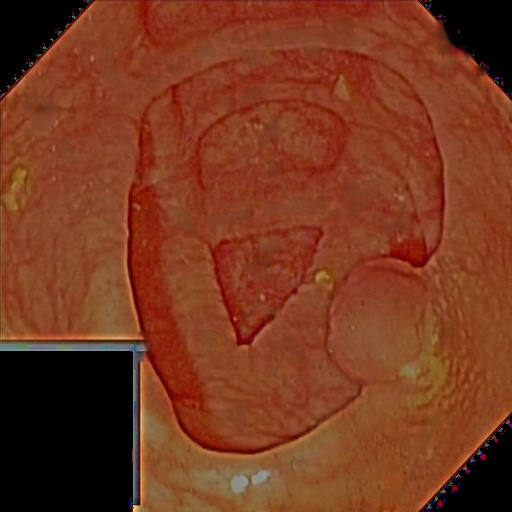
\includegraphics[width=0.25\columnwidth]{libs/out2.png_inpainted.jpg} };
    %                   \node[text width=2.5cm] at (-3.0, -3.0) {\small\textit{a) Antidistorted Image}};
    %                   \pause
    %                   \node (ref1)  at (0,0){
    %                       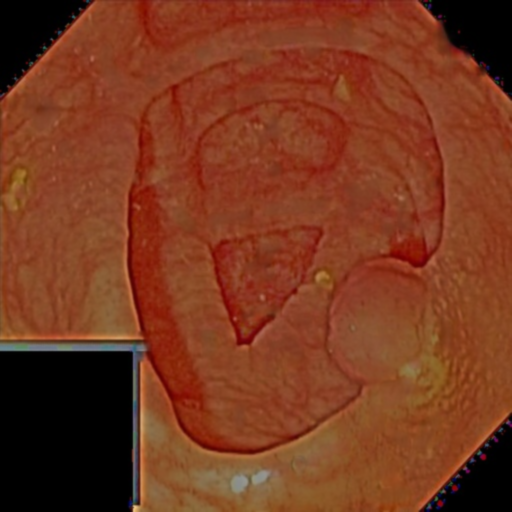
\includegraphics[width=0.25\columnwidth]{libs/defocus_sigma_0.75.png} };
    %                   \path[draw=magenta,thick,->]<1-> (in) to  (ref1);
    %                   \node[text width=2.5cm] at (0.0, -3.0) {\small\textit{b) Blured image with Defocus Blur $b \sim N(0, \sigma^2_b=(0.75)^2)$ }};
    %                   \pause
    %                   \node (noisy1)  at (3,0){
    %                       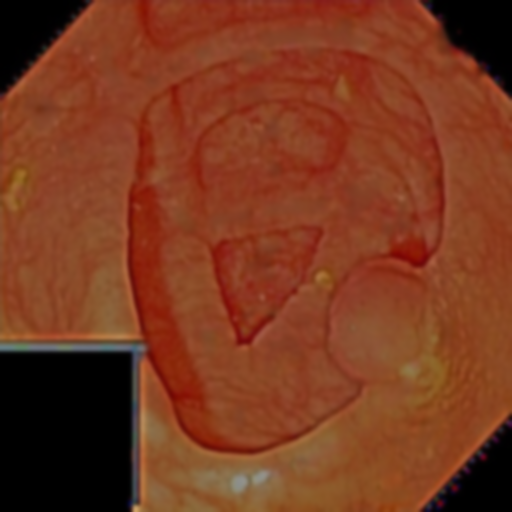
\includegraphics[width=0.25\columnwidth]{libs/defocus_sigma_2.png} };
    %                   \node[text width=2.5cm] at (3.0, -3.0) {\small\textit{c) Blured image with Defocus Blur $b \sim N(0, \sigma^2_b=(2)^2)$ }};
    %                   \path[draw=magenta,thick,->]<1-> (in) to [bend right] (noisy1);


    %               \end{tikzpicture}}
    %         %   }


    % \end{itemize}
    \begin{figure}
        \centering
        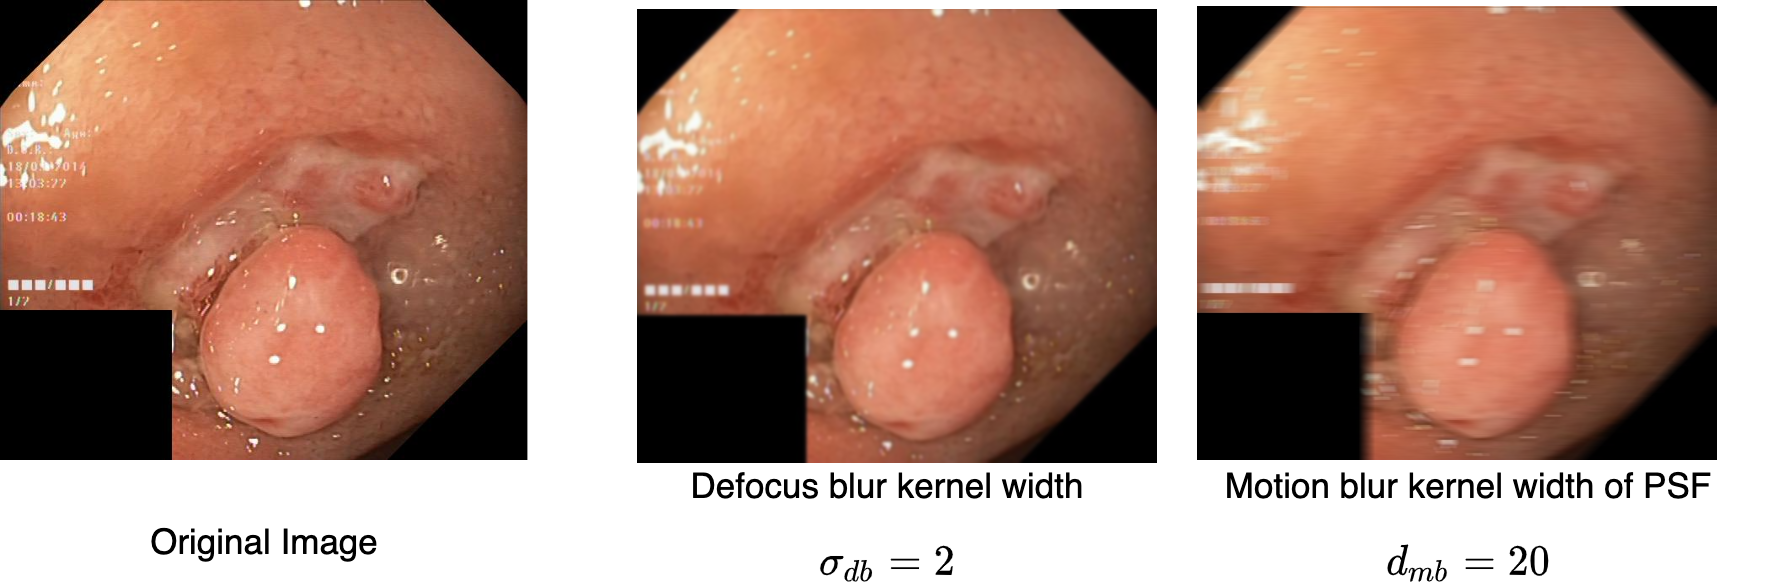
\includegraphics[width=1\textwidth]{libs/bluraddres2.png}
        \caption{Bluring image with Defocus Blur $b \sim N(0, \sigma^2_{db})$ and motion blur PSF kernel width $l_{mb}$}
        \label{blur_inpainted}
    \end{figure}
\end{frame}

\begin{frame}{Result images after adding Uneven Illumination}

    % % \begin{itemize}
    %     % {\item Uneven Illumination\\

    %           \begin{tikzpicture}[remember picture]

    %               \node (in)  at (0,0){
    %                   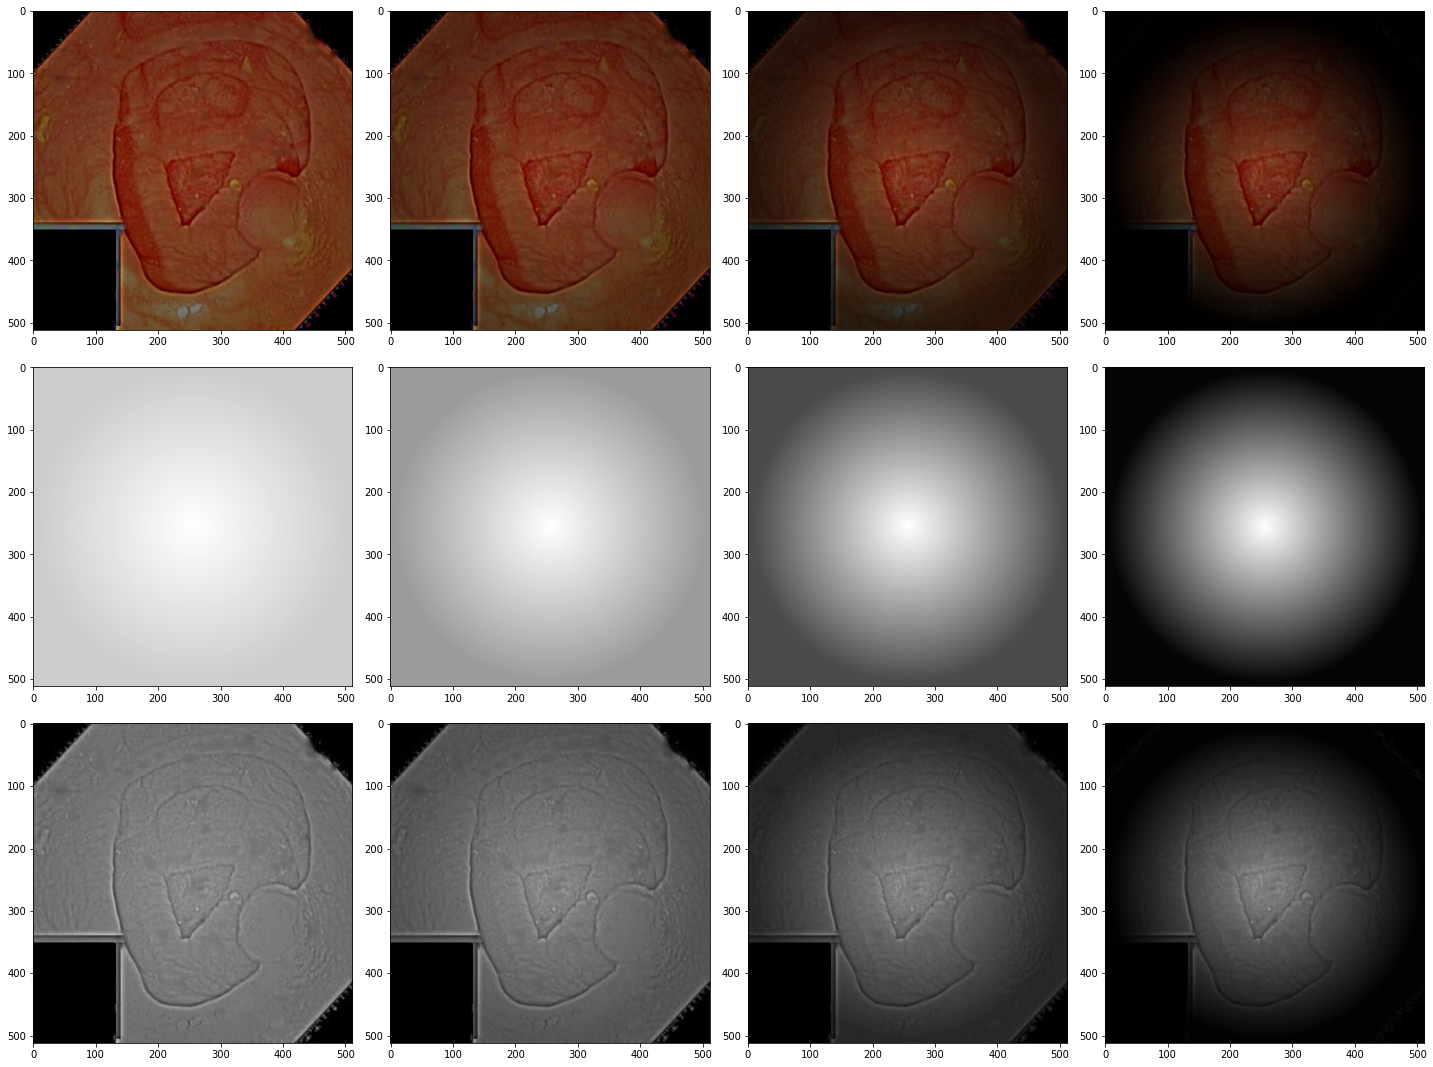
\includegraphics[width=0.8\columnwidth]{libs/unevencreate.png} };
    %               \node at (0.0, -3.5) {\small\textit{Artificial Uneven Illumination process}};



    %           \end{tikzpicture}
    %         %   }



    % \end{itemize}
    \begin{figure}[h]
        \begin{center}
            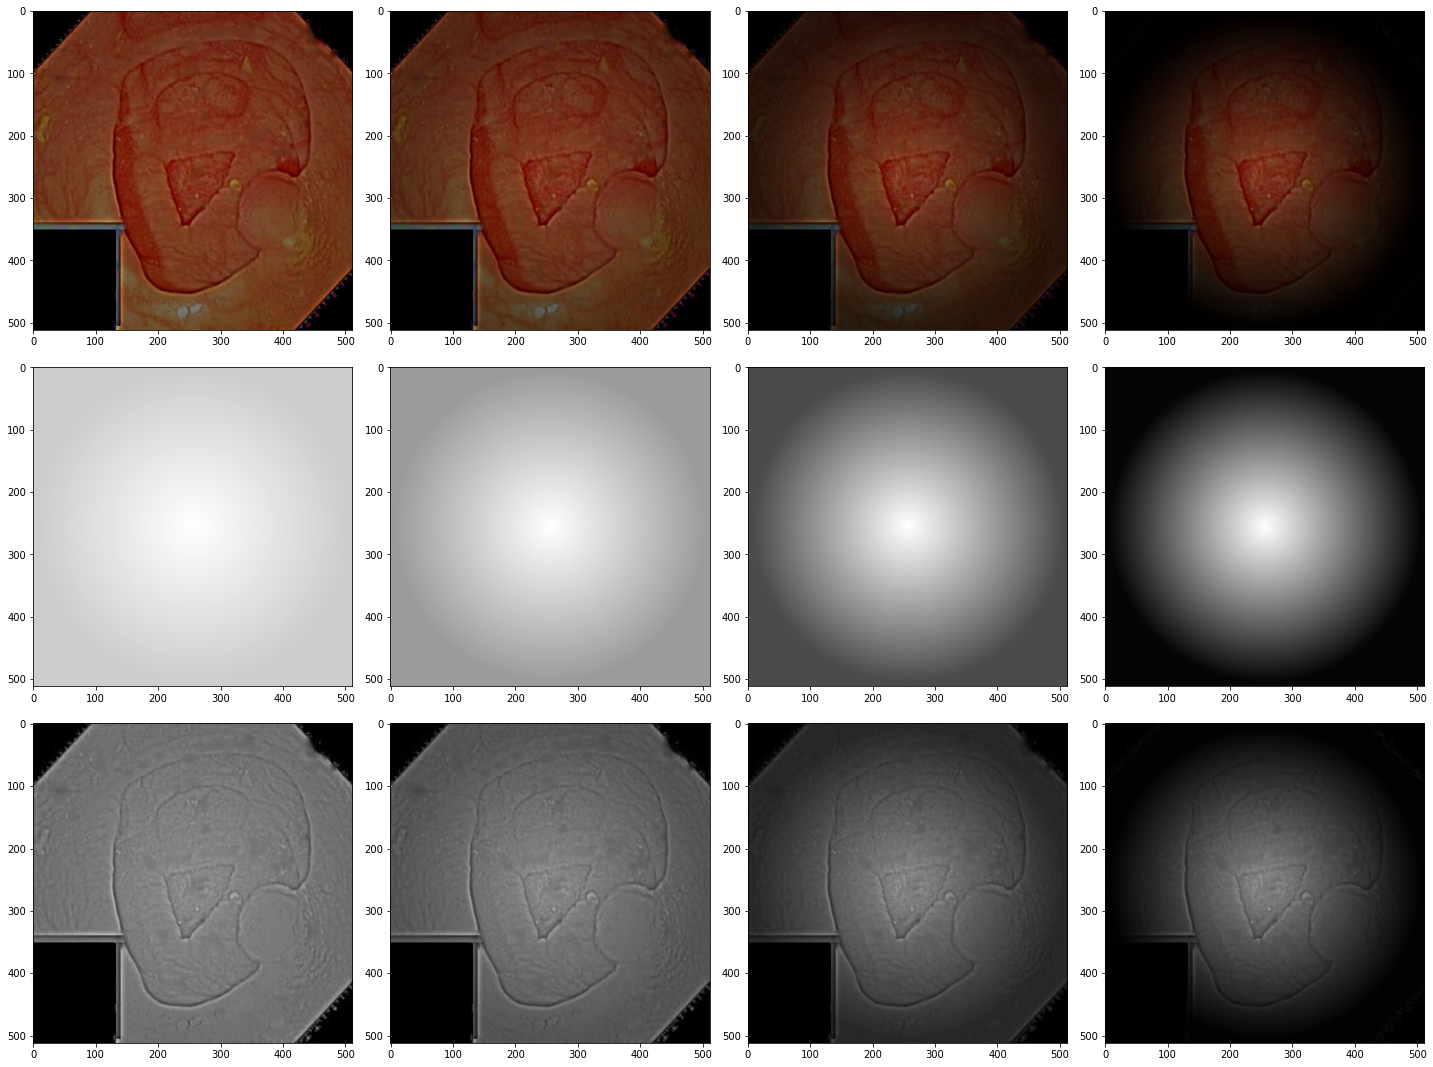
\includegraphics[width=0.8\columnwidth]{libs/unevencreate.png}
            \caption{Artificial Uneven Illumination process. The first row is the result after adding the mask (second row) into the V-channel of image (third row).}
        \end{center}
    \end{figure}
\end{frame}

\begin{frame}{Result images after adding Specular Reflection}

    % % \begin{itemize}
    %     % \only<1-3>{\item Specular Reflection\\
    %           \only<1-3>{
    %               \begin{tikzpicture}[remember picture]

    %                   \node (in)  at (-3,0){
    %                       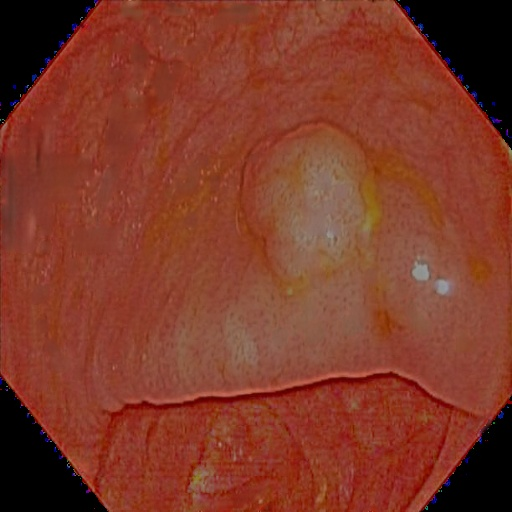
\includegraphics[width=0.2\columnwidth]{libs/out3.png_inpainted.jpg} };
    %                   \node[text width=2.5cm] at (-3.0, -3.0) {\small\textit{a) Antidistorted Images}};
    %                   \pause
    %                   \node (ref1)  at (3,0){
    %                       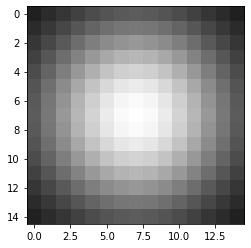
\includegraphics[width=0.2\columnwidth]{libs/srmask.png} };
    %                   \path[draw=magenta,thick,->]<1-> (ref1) to [bend left] (in);
    %                   \pause
    %                   \node (noisy1)  at (0,0){
    %                       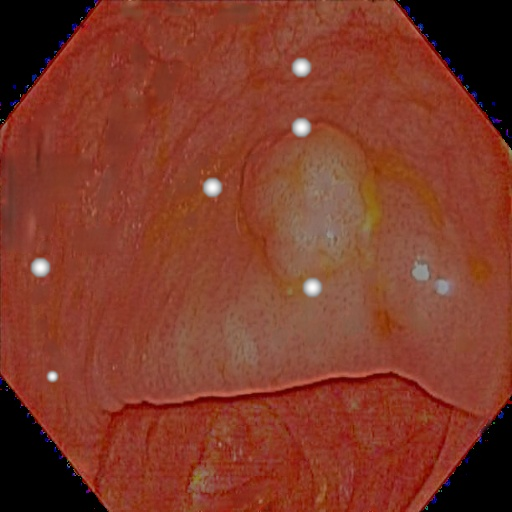
\includegraphics[width=0.2\columnwidth]{libs/srres.png} };
    %                   \node[text width=2.5cm] at (0.0, -3.0) {\small\textit{b) Artificial Specular Reflection Image}};
    %                   \path[draw=magenta,thick,->]<1-> (in) to  (noisy1);


    %               \end{tikzpicture}}
    %         %   }


    % % \end{itemize}
    \begin{figure}
        \centering
        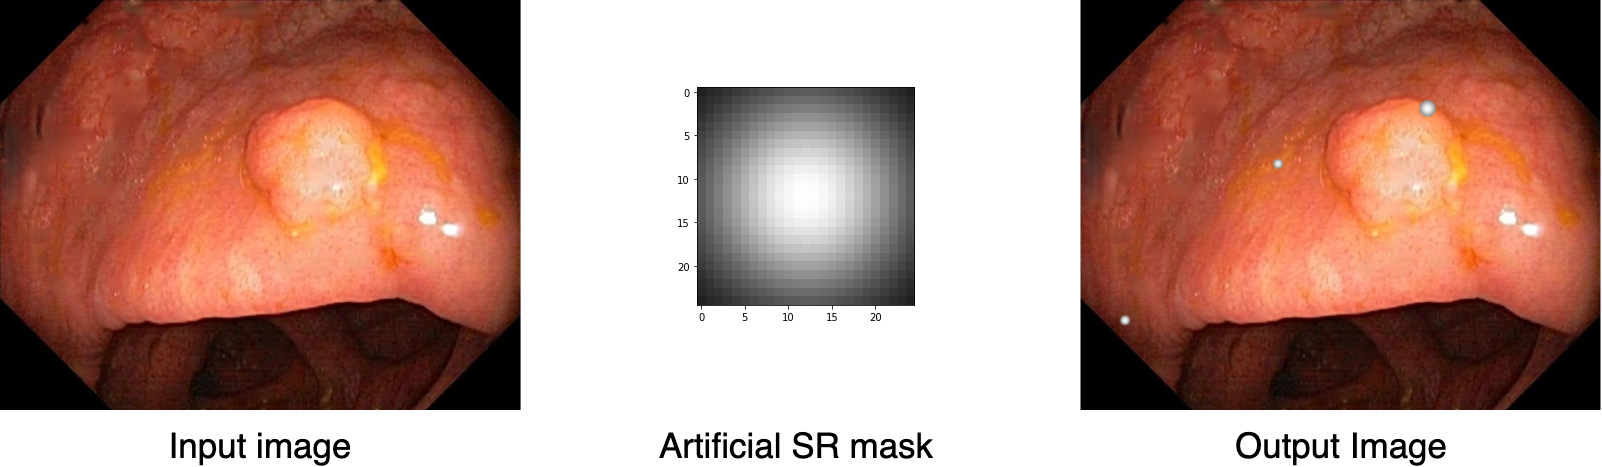
\includegraphics[width=1\textwidth]{libs/srres4.png}
        \caption{Artificial Specular Reflection by using the artificial PSF with the random position}
        \label{sr_inpainted}
    \end{figure}
\end{frame}

%% ---------------------------------------------------------------------------
% Reference frames
\begin{frame}[shrink=50]
    \frametitle{References}
    \printbibliography
\end{frame}

%% ---------------------------------------------------------------------------
% Final frame
\begin{frame}{}
    \centering
    \huge{\textbf{\example{Thank you for watching!}}}

    \vspace{1cm}

    \Large{\textbf{Contact:}}
    \newline
    \vspace*{0.5cm}
    \large{\email{tansy.nguyen@math.univ-paris13.fr}}
\end{frame}

\end{document}